\documentclass[xcolor=pdftex, x11names,table]{book}
 % Paquete de estilo 
%--------------------------------------------------------------------------
% ARCHIVO .TEX DE DISEÑO
% PAQUETES Y ESTILO DEL LIBRO 
%--------------------------------------------------------------------------
% Paquetes 
\usepackage[english,spanish]{babel}
\usepackage[latin1]{inputenc}                      % Entrada de acentos
\usepackage[T1]{fontenc}
\usepackage[autostyle, spanish = mexican]{csquotes}% manejo de comillas: " "
\MakeOuterQuote{"}
\usepackage{pslatex}                              % Fuentes finas postscript
%\usepackage[sc]{mathpazo}                         % Fuentes mathpazo
\usepackage{helvet}
\linespread{1.05}                                  % Fuente Palatino necesita espaciado
\usepackage[full]{textcomp}                        % Caracteres especiales como ' (recto)
\usepackage{xcolor}                                % Color: X11names (en el documentclass)
% COLORES personales---------------------------------------------------
    \definecolor{colortitulo}{RGB}{11,17,79} % 
    \definecolor{colordominante}{RGB}{11,17,79}
    \definecolor{colordominanteF}{RGB}{219,68,14}
    \definecolor{colordominanteD}{RGB}{137,46,55}
    \definecolor{mostaza}{RGB}{231,196,25}
    \definecolor{amarilloM}{RGB}{248,199,90}
    \definecolor{amarilloD}{RGB}{251,237,121}
    \definecolor{azulF}{rgb}{.0,.0,.3}
    \definecolor{grisD}{rgb}{.3,.3,.3}
    \definecolor{grisF}{rgb}{.6,.6,.6}
    \definecolor{grisamarillo}{RGB}{248,248,245} 
    \definecolor{miverde}{RGB}{44,162,67}
    \definecolor{verdep}{RGB}{166,206,58}
    \definecolor{verdencabezado}{RGB}{166,206,58}
    \definecolor{verdeF}{RGB}{5,92,8}
    \definecolor{azul1}{RGB}{20,60,102}
    \definecolor{rojo1}{RGB}{154,20,65}
    \colorlet{mygray}{black!20}
    \newcommand{\verde}{\color{miverde}}
% Fin COLORES personales-------------------------------------------------
%\usepackage{psboxit}
\usepackage{pstricks}
\usepackage{xparse}
\usepackage{tcolorbox} 
\tcbuselibrary{skins,breakable}                    % Librerías tcolorbox
\usepackage{tikz,tkz-tab}% Cajas de Teoremas, ejemplos, etc.
\usetikzlibrary{positioning,shadows,backgrounds,calc}%
\usepackage{tikzpagenodes}
\usepackage{xargs}                                 % Comandos con opciones
\DeclareGraphicsExtensions{.pdf,.png,.jpg}
\usepackage{multicol}
% %\usepackage{epstopdf}% Conversión - Miktes 2.9 o inferior, TexLive 2009. o inferior
\usepackage[small,bf]{caption}
\usepackage[breaklinks,colorlinks=true, pdfstartview=FitV, linkcolor=azulF, citecolor=azulF, urlcolor=azulF]{hyperref}
\usepackage{amsmath,amssymb,amsfonts,latexsym,cancel,stmaryrd}%
\usepackage[ruled,,vlined,lined,linesnumbered,algochapter]{algorithm2e}
\usepackage{framed}
\usepackage{titletoc}
\usepackage{calc}
\usepackage{colortbl} 
\usepackage{tabularx}
\usepackage{fancyvrb}
%\usepackage{minted}   %habilitar solo en Ubuntu (Linux)
\usepackage{array}
\usepackage{wasysym}
\usepackage{supertabular}
\usepackage{booktabs}
\usepackage[shortlabels]{enumitem}

%----------------------------------------------------------------------------------------
% Fuentes
%----------------------------------------------------------------------------------------
% Comandos para fuentes especiales
\newcommandx*{\fnte}[4][1=pag,2=9,3=n]{{\color{azulF}\fontfamily{#1}
\fontsize{#2}{1}\fontshape{#3}\selectfont{#4}}}

\newcommandx*{\fntb}[4][1=pag,2=9,3=n]{{\color{azulF}\fontfamily{#1}\fontsize{#2}{1}\fontseries{b}\fontshape{#3}\selectfont{#4}}}

\newcommandx*{\fntg}[4][1=pag,2=9,3=n]{{\color{grisF}\fontfamily{#1}\fontsize{#2}{1}\fontshape{#3}\selectfont{#4}}}

\newcommand{\fhv}[2]{{\fontfamily{pag}\fontsize{#1}{1}\selectfont{#2}}}

\newcommand{\fhvb}[2]{{\fontfamily{pag}\fontseries{b}\fontsize{#1}{1}\selectfont{#2}}}
% Fin fuentes----------------------------------------------------------

%********************************** DISENO *************************************

%----------------------------------------------------------------------------------------
% Cabeceras
%----------------------------------------------------------------------------------------
\usepackage{fancyhdr}

% Números de página en rectángulos y capítulo. Necesitamos posicionar los nodos
\usepackage[absolute]{textpos}
    \setlength{\TPHorizModule}{10mm}% 1 generic horizontal unit is equivalent to 10mm
    \setlength{\TPVertModule}{10mm}% 1 generic vertical unit is equivalent to 10mm
    \textblockorigin{0mm}{0mm}% top left corner set as origin

%------------------------------------------------------------------------------
% Decoración de cabeceras 
% Texto en secciones
\newcommand{\helvb}{%
\fontfamily{phv}\fontseries{b}\fontsize{9}{11}\selectfont}
\newcommand{\helv}{%
\fontfamily{phv}\fontsize{9}{11}\selectfont}
\renewcommand{\sectionmark}[1]{\markright{\thesection\hspace{5pt}#1}{}} 
% Configuración de fuentes para el número de página en el encabezado
\fancyhf{} 
%OP 1: Todas las páginas con la sección a la izquierda
%\fancyhead[LO,LE]{\rightmark} % L=Left, O=Odd y  E=Even pages
%OP 2: Todas las páginas con la sección a la izquierda en un rectángulo (todo el header)

\fancyhead[LO,LE]{\helv\rightmark
\begin{textblock}{1}(0,0)
\begin{tikzpicture}[remember picture,overlay]
  %\fill[grisamarillo] (current page.north west) 
  \fill[verdencabezado,opacity=0.7] (current page.north west) 
  rectangle
  ([xshift=2pt,yshift=-3pt]current page.east|-current page header area.south east);
\end{tikzpicture}
\end{textblock}
}
% Fin decoración cabeceras

\renewcommand{\headrulewidth}{0pt}   % Ancho de la línea bajo el encabezado
\addtolength{\headheight}{2.5pt}     % Aumente el espacio alrededor de la cabecera 
\renewcommand{\footrulewidth}{0pt}   % Elimina la línea en el pie de página
% Estilo para cuando se especifica "pagestyle plain"
\fancypagestyle{plain}{\fancyhead{}\renewcommand{\headrulewidth}{0pt}} 

% Elimina el encabezado de las páginas impares vacías al final de los capítulos
\makeatletter
\renewcommand{\cleardoublepage}{
\clearpage\ifodd\c@page\else
\hbox{}
\vspace*{\fill}
\thispagestyle{empty}
\newpage
\fi}
\makeatother

% Números de página en el borde
\fancyfoot[LO]{
\begin{textblock}{3}(21,1) % y=1 inch = margen
\begin{tikzpicture}[overlay]
\node[draw=colordominante!10,
rectangle,minimum width=1.5cm, minimum height=1.5cm,
anchor=west,
fill=colordominante!10,font=\fontsize{20}{1}\sffamily\bfseries,inner sep=4pt,outer sep=4pt] 
at (-1.5cm,0pt){\textcolor{mycolorA}{\thepage}};
\end{tikzpicture}
\end{textblock}
}

\fancyfoot[RE]{
\begin{textblock}{3}(18,1)% y=1 inch = margen
\begin{tikzpicture}[overlay]
\node[draw=colordominante,
rectangle,minimum width=2cm, minimum height=2cm,
anchor=west,
fill=colordominante,font=\fontsize{25}{1}\sffamily\bfseries,inner sep=2pt,outer sep=2pt] 
at (-1.5cm,0pt){\textcolor{gray!10}{\thepage}};   
\end{tikzpicture}
\end{textblock}
}
%-- Fin cabeceras 

%----------------------------------------------------------------------------------------
% Color en los márgenes
%----------------------------------------------------------------------------------------
% \pagecolor{grisamarillo}
% \usepackage{eso-pic}
% \pagecolor{grisamarillo}
% \AddToShipoutPictureBG{%
%  \AtTextLowerLeft{\color{grisamarillo}%
%   \rule[-\footskip]{\textwidth}{\dimexpr\textheight+\footskip}}}

% Fin color márgenes



%----------------------------------------------------------------------------------------
% Prólogo
%----------------------------------------------------------------------------------------
\NewDocumentEnvironment{prologo}{O{}}{%
\addcontentsline{toc}{schapter}{%
\hspace{6em}{\color{azulF}{\fontfamily{phv}\fontsize{9}{10}\selectfont Prol\'ogo}} \qquad}
\chapter*{Prólogo}
\smallskip\smallskip
\begin{minipage}{0.9\textwidth}
 #1}{\end{minipage}}
 

%----------------------------------------------------------------------------------------
% Título
%----------------------------------------------------------------------------------------
\newcommand*{\titulo}[4]{\begingroup%
\raggedleft 
\vspace*{\baselineskip} % Espacio en blanco en la parte superior de la página
{\Large #1}\\[0.167\textheight] % Autor
{\LARGE\bfseries #2}\\[\baselineskip] % pre-título
{\textcolor{colortitulo}{\Huge #3}}\\[\baselineskip] % Título
{\Large \textit{#4}}\par % Descripción adicional

\vfill % Espacio en blanco entre el bloque de título y "la editorial"

{\raggedright
\begin{minipage}[c]{0.08\textwidth}
\raisebox{-2.0cm}{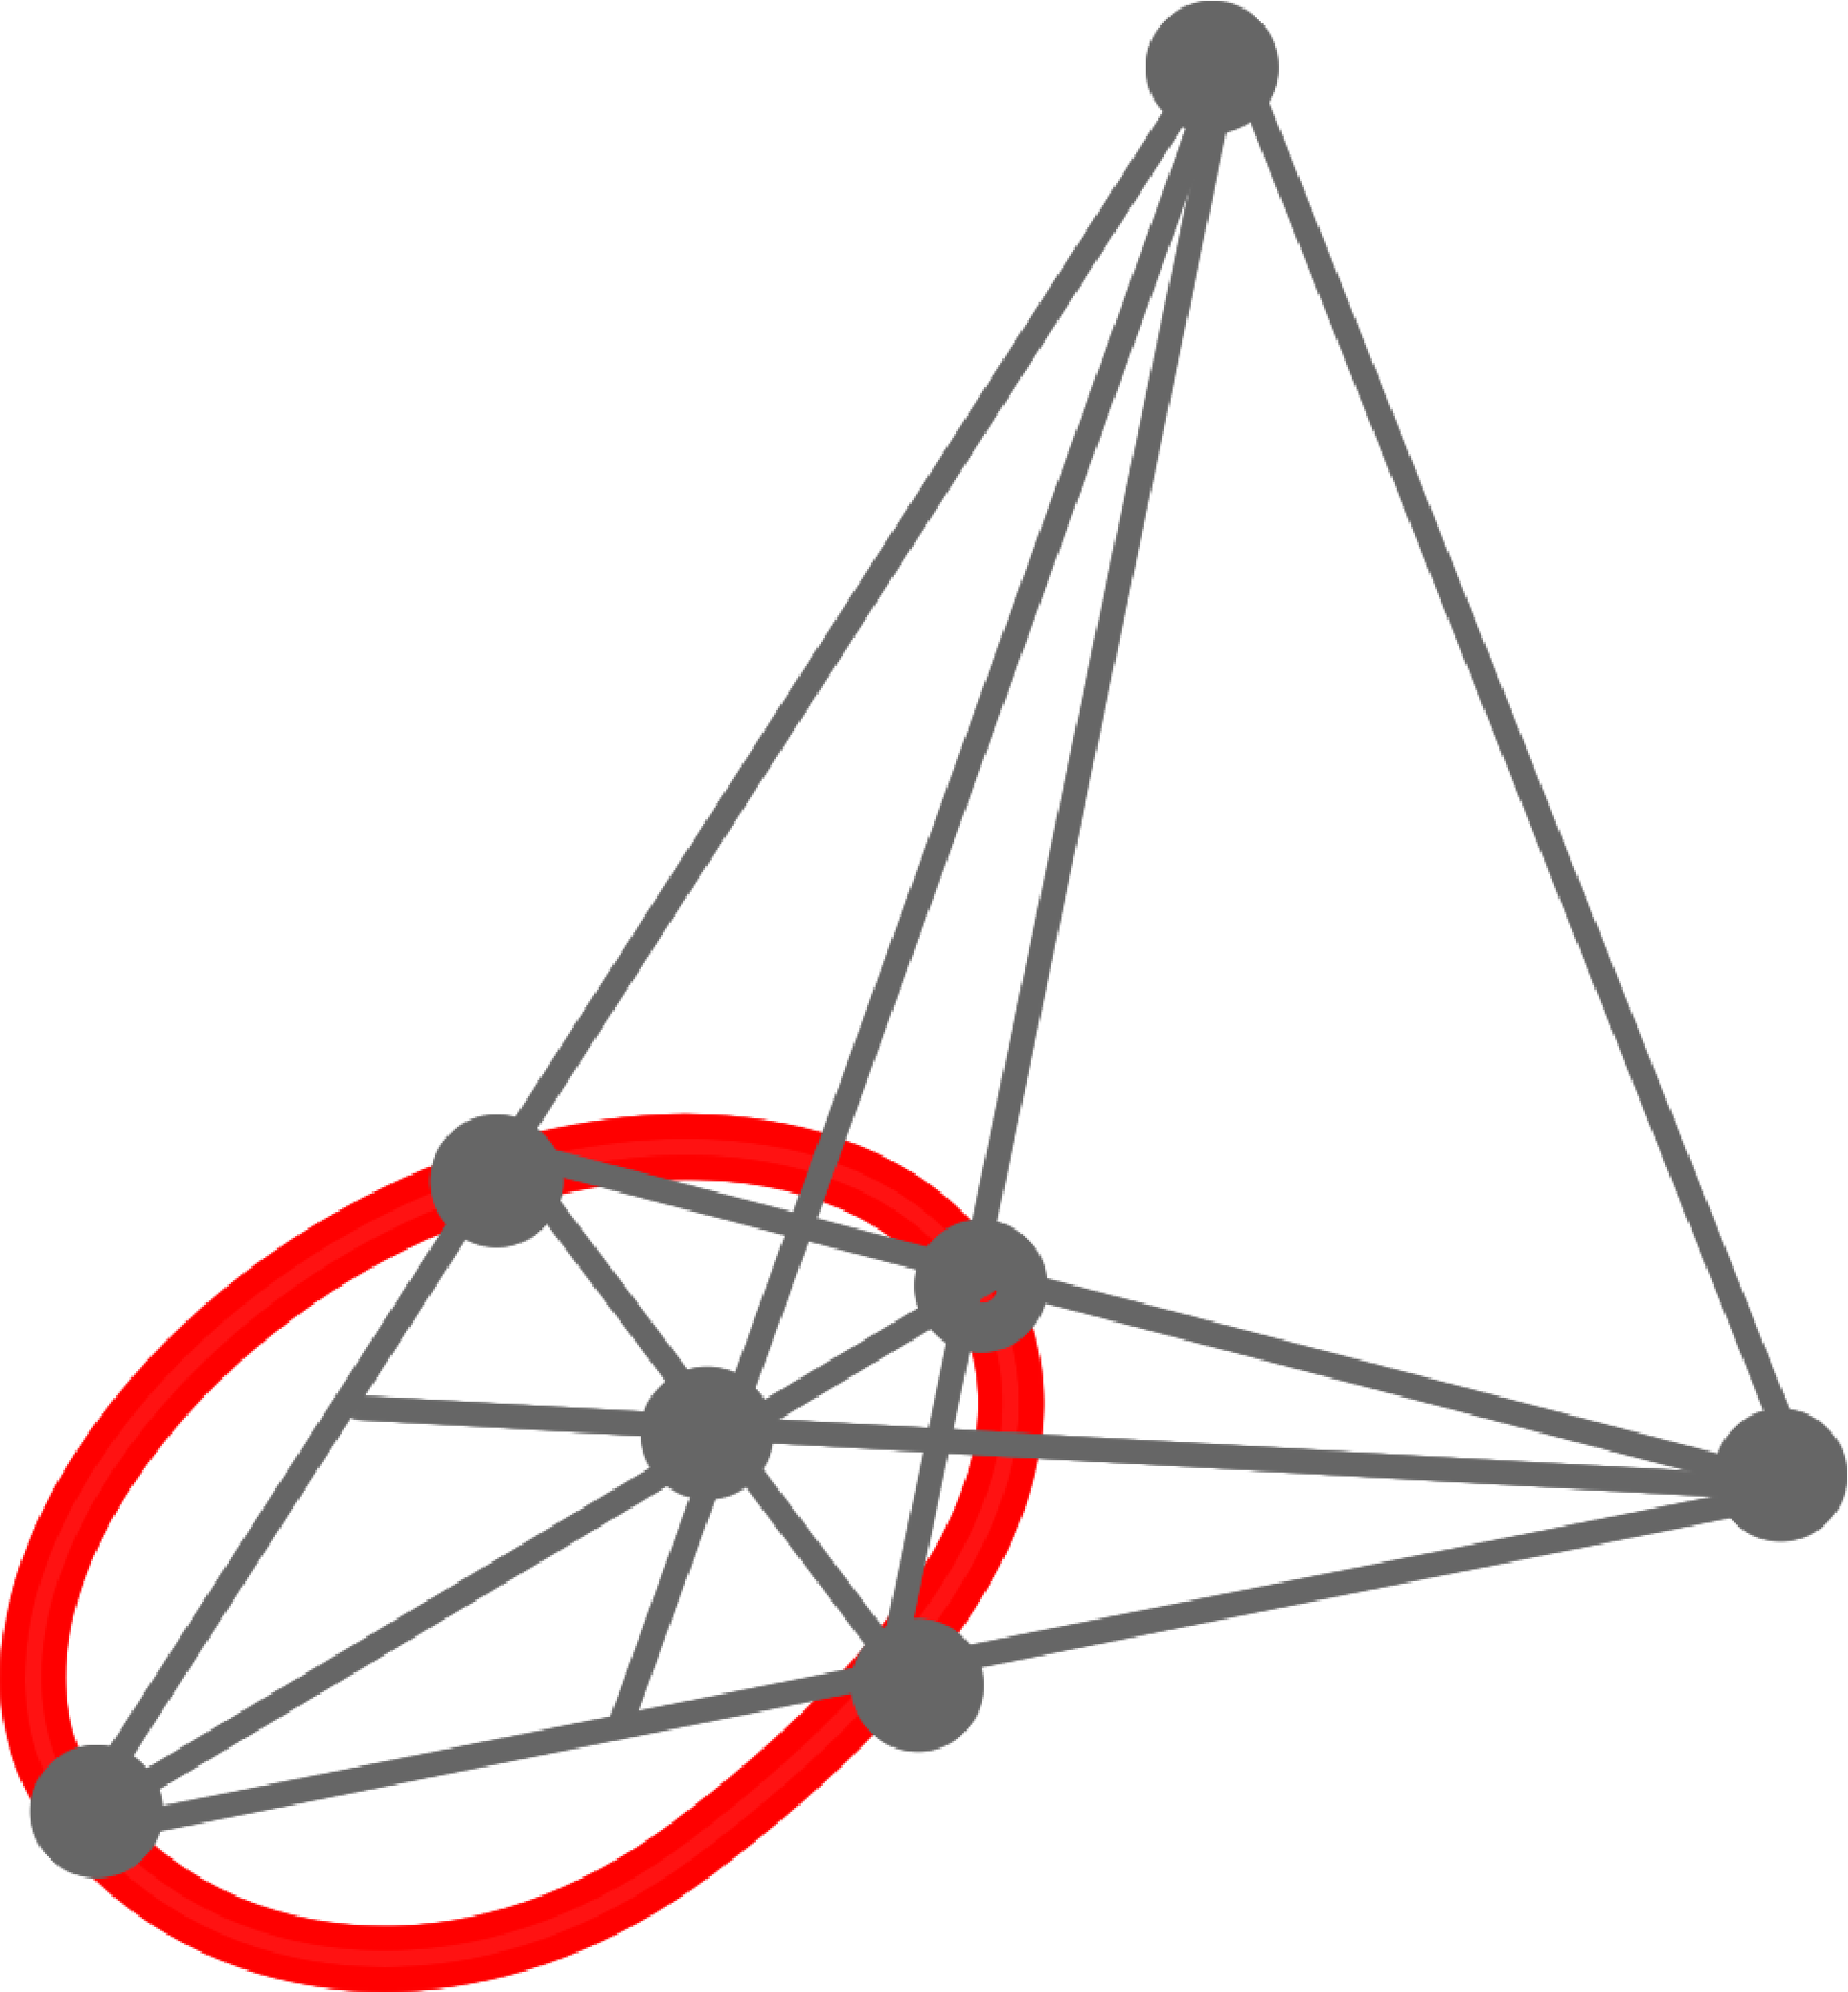
\includegraphics[width=1.4cm]{images/logo}}
 \end{minipage}
\  \ \hfill\begin{minipage}[t]{0.9\textwidth}
{\color{gray}
 \fhv{9}{Digital}\\
 \fhvb{9}{\color{azulF}Educación e Internet.}
  \fntg[pag][8]{\color{grisF}
  \href{http://www.ecampus.usfx.bo/).}}}
\end{minipage}          
}%raggedright
\vspace*{3\baselineskip} % Espacio en blanco antes del final de página
\endgroup}
% Fin Titulo--------------------------------------------------------


%----------------------------------------------------------------------------------------
% Copypright, ISBN, ...
%----------------------------------------------------------------------------------------
\def\copyrightpage{\thispagestyle{empty}%
\vbox to\textheight\bgroup\vfill\obeylines\obeyspaces\xcopyrightpage}

\def\xcopyrightpage#1#2\end#3{\scriptsize\parindent=0pt
Copyright\copyright{#1} 
\vskip40pt
#2\vskip200pt\egroup\endgroup}
\let\endcopyrightpage\relax
% Fin Copyright



%-------------------CONTENIDO -----------------------------------------------------
\definecolor{mycolorA}{RGB}{0,133,202}  % 
\definecolor{mycolorB}{RGB}{166,206,58} % 

% patching of \tableofcontents to use sans serif font for the tile
\patchcmd{\tableofcontents}{\contentsname}{\contentsname}{}{}
% patching of \@part to typeset the part number inside a framed box in its own line
% and to add color
\makeatletter
\patchcmd{\@part}
  {\addcontentsline{toc}{part}{\thepart\hspace{1em}#1}}
  {\addtocontents{toc}{\protect\addvspace{20pt}}
    \addcontentsline{toc}{part}{\huge{\protect\color{colordominante}%
      \setlength\fboxrule{2pt}\protect\Circle{%
        \hfil\thepart\hfil%
      }%
    }\\[2ex]\color{colordominante}\sffamily\large#1}}{}{}
\makeatother

% this is the environment used to typeset the  entries in the ToC
% it is a modification of the leftbar environment of the framed package
\renewenvironment{leftbar}
  {\def\FrameCommand{\hspace{6em}%
    {\color{mycolorB}\vrule width 2pt depth 6pt}\hspace{1em}}%
    \MakeFramed{\parshape 1 0cm \dimexpr\textwidth-6em\relax\FrameRestore}\vskip2pt%
  }
 {\endMakeFramed}

% using titletoc we redefine the ToC entries for parts, chapters, sections, and subsections
\titlecontents{part}
  [0em]{\centering}
  {\contentslabel}
  {}{}
\titlecontents{chapter}
  [0em]{\vspace*{2\baselineskip}}
  {\parbox{4.5em}{%
    \hfill\Huge\bfseries\color{mycolorA}\thecontentspage}%
   \vspace*{-2.3\baselineskip}\leftbar{\fhvb{12}{\chaptername~\thecontentslabel}}\\}
  {}{\endleftbar}
\titlecontents{section}
  [8.4em]
  {\sffamily\contentslabel{3em}}{}{}
  {\hspace{0.5em}\nobreak\itshape\color{mycolorA}\contentspage}
\titlecontents{subsection}
  [8.4em]
  {\sffamily\contentslabel{3em}}{}{}  
  {\hspace{0.5em}\nobreak\itshape\color{mycolorA}\contentspage}

% Fin Contenido 

%----------------------------------------------------------------------------------------
% CAPITULO Estilo simple
%----------------------------------------------------------------------------------------
 \usepackage{titlesec, blindtext, color}
 \newcommand{\hsp}{\hspace{10pt}}
 \titleformat{\chapter}[hang]{\large\bfseries}{{
         \fontsize{5em}{5em}\selectfont\black
         \thechapter}\hsp\textcolor{verdep}{\vrule height 3em width 1pt}\hsp}{0pt}{\LARGE\bfseries\color{mycolorA}}


%----------------------------------------------------------------------------------------
%	Numeración de las secciones -- en el margen
%----------------------------------------------------------------------------------------

\makeatletter
\renewcommand{\@seccntformat}[1]{\llap{\textcolor{verdeF}{\csname the#1\endcsname}\hspace{1em}}}                    
\renewcommand{\section}{\@startsection{section}{1}{\z@}
{-4ex \@plus -1ex \@minus -.4ex}
{1ex \@plus.2ex }
{\normalfont\large\sffamily\bfseries}}
\renewcommand{\subsection}{\@startsection {subsection}{2}{\z@}
{-3ex \@plus -0.1ex \@minus -.4ex}
{0.5ex \@plus.2ex }
{\normalfont\sffamily\bfseries}}
\renewcommand{\subsubsection}{\@startsection {subsubsection}{3}{\z@}
{-2ex \@plus -0.1ex \@minus -.2ex}
{0.2ex \@plus.2ex }
{\normalfont\small\sffamily\bfseries}}                        
\renewcommand\paragraph{\@startsection{paragraph}{4}{\z@}
{-2ex \@plus-.2ex \@minus .2ex}
{0.1ex}
{\normalfont\small\sffamily\bfseries}}
\makeatother
% Fin numeración secciones



%---------------------------------------------------------------------------------
%  Entornos:  Ejemplo, teorema, proposición, lema, lista de ejercicios, 
%              interludio, caja simple  
%---------------------------------------------------------------------------------

%  Cajas con el paquete  tcbcolor
%  CONTADORES: ejemplo, definicion, lema, teorema, corolario, proposicion,ejercicio 
\newcounter{tcbteo}[chapter]
\renewcommand{\thetcbteo}{\thechapter.\arabic{tcbteo}}

\newcounter{tcbdefi}[chapter]
\renewcommand{\thetcbdefi}{\thechapter.\arabic{tcbdefi}}

\newcounter{tcblema}[chapter]
\renewcommand{\thetcblema}{\thechapter.\arabic{tcblema}}

\newcounter{tcbcoro}[chapter]
\renewcommand{\thetcbcoro}{\thechapter.\arabic{tcbcoro}}

\newcounter{tcbvoca}[chapter]
\renewcommand{\thetcbvoca}{\thechapter.\arabic{tcbvoca}}

%  \newcounter{tcbListaEjercicios}[chapter]
%  \renewcommand{\thetcbListaEjercicios}{\thechapter.\arabic{tcbListaEjercicios}}

\newcounter{tcbpropo}[chapter]
\renewcommand{\thetcbpropo}{\thechapter.\arabic{tcbpropo}}

\newlength{\examlen}
\tikzset{
    wnodeTeorema/.style={%
         rectangle,  top color=gray!5, bottom color=gray!5,
         inner sep=1mm,anchor=west,font=\small\bf\sffamily},
     wnodeEjercicios/.style={%
     	rectangle,  top color=gray!15, bottom color=gray!15,
     	inner sep=1mm,anchor=west,font=\small\bf\sffamily},
   wnodeminimo/.style={%
         rectangle,  top color=white, bottom color=white,
         text=azulF,inner sep=1mm,anchor=west,font=\small\bf\sffamily}      
}



%\begin{teorema}  o \begin{teorema}[de tal] o \begin{teorema}[][ref]
% Teorema -----------------------------------------------------
\newtcolorbox{wwteorema}[3][]{%
arc=0mm,breakable,enhanced,colback=gray!5,boxrule=0pt,top=7mm,
fontupper=\normalsize,step and label={tcbteo}{#3},
overlay unbroken = {\draw[color=colordominante,line width=0.2pt] (frame.north west)--([xshift=0pt]frame.north east);
%Caja de Título: teo --
\node[wnodeTeorema](tituloteo) at ([xshift=0pt, yshift=-4mm]frame.north west)
{\textbf{\color{colordominante} Teorema \thetcbteo \;#2}};
%Borde superior --
\draw[colordominante,line width=2.5cm] ([xshift=1.25cm, yshift=0cm]frame.north west)-- +(\examlen,3pt);
},%
overlay first = {\draw[color=colordominante,line width=0.2pt] (frame.north west)--([xshift=0pt]frame.north east);
%Caja de Título: teo --
\node[wnodeTeorema](tituloteo) at ([xshift=0pt, yshift=-4mm]frame.north west)
{\textbf{\color{colordominante} Teorema \thetcbteo \;#2}};
%Borde superior --
\draw[colordominante,line width=2.5cm] ([xshift=1.25cm, yshift=0cm]frame.north west)-- +(\examlen,3pt);
},%
% Mantener borde en cambio de página 
overlay last = {\draw[color=colordominante,line width=0.2pt] (frame.north west)--([xshift=0pt]frame.north east);
                } 
#1}
%-
\NewDocumentEnvironment{teorema}{O{} O{} O{}}{\smallskip\begin{wwteorema}{#1}{#2}%
 #3}{\end{wwteorema}\smallskip }
% TEOREMA---------------------------------------------------------

%%%%%%%%%%%%%%%%%%%
%%%%%%%%%%%%%%%%%%%

% Ejemplos -----------------------------------------------------
\newtcolorbox{wwejem}[3][]{%
	arc=0mm,breakable,enhanced,colback=gray!15,boxrule=0pt,top=7mm,
	fontupper=\large,step and label={tcbejem}{#3},
	overlay unbroken ={\draw[color=colordominante,line width=0.2pt] (frame.north west)--([xshift=0pt]frame.north east);
		%Caja de Título: ejem --
		\node[wnodeEjercicios](tituloteo) at ([xshift=0pt, yshift=-4mm]frame.north west)
		{\textbf{\color{azul1} {\large Ejemplos: }}};
		%Borde superior --
		\draw[colordominante,line width=2.5cm] ([xshift=1.25cm, yshift=0cm]frame.north west)-- +(\examlen,3pt);
	}, %
	overlay first ={\draw[color=colordominante,line width=0.2pt] (frame.north west)--([xshift=0pt]frame.north east);
		%Caja de Título: ejem --
		\node[wnodeTeorema](tituloteo) at ([xshift=0pt, yshift=-4mm]frame.north west)
		{\textbf{\color{colordominante} Ejemplos:}};
		%Borde superior --
		\draw[colordominante,line width=2.5cm] ([xshift=1.25cm, yshift=0cm]frame.north west)-- +(\examlen,3pt);
	}, %
	% Mantener borde en cambio de página 
	overlay last ={\draw[color=colordominante,line width=0.2pt] (frame.north west)--([xshift=0pt]frame.north east);
	},
	#1}
%-
\NewDocumentEnvironment{ejemplos}{O{} O{} O{}}{\smallskip\begin{wwejem}{#1}{#2}%
		#3}{\end{wwejem}\smallskip }
% ---------------------------------------------------------



%%%%%%%%%%%%%%%%%%%
%%%%%%%%%%%%%%%%%%%

%\begin{proposicion}  o \begin{proposicion}[de tal] o \begin{proposicion}[][ref]
% Proposición-----------------------------------------------------
\newtcolorbox{wwpropo}[3][]{%
arc=0mm,breakable,enhanced,colback=gray!5,boxrule=0pt,top=7mm,
fontupper=\normalsize,step and label={tcbpropo}{#3},
overlay unbroken ={\draw[color=colordominante,line width=0.2pt] (frame.north west)--([xshift=0pt]frame.north east);
%Caja de Título: propo --
\node[wnodeTeorema](tituloteo) at ([xshift=0pt, yshift=-4mm]frame.north west)
{\textbf{\color{colordominante} Proposición \thetcbpropo\;#2}};
%Borde superior --
\draw[colordominante,line width=2.5cm] ([xshift=1.25cm, yshift=0cm]frame.north west)-- +(\examlen,3pt);
}, %
overlay first ={\draw[color=colordominante,line width=0.2pt] (frame.north west)--([xshift=0pt]frame.north east);
%Caja de Título: propo --
\node[wnodeTeorema](tituloteo) at ([xshift=0pt, yshift=-4mm]frame.north west)
{\textbf{\color{colordominante} Proposición \thetcbpropo\;#2}};
%Borde superior --
\draw[colordominante,line width=2.5cm] ([xshift=1.25cm, yshift=0cm]frame.north west)-- +(\examlen,3pt);
}, %
% Mantener borde en cambio de página 
overlay last ={\draw[color=colordominante,line width=0.2pt] (frame.north west)--([xshift=0pt]frame.north east);
        },
#1}
%-
\NewDocumentEnvironment{proposicion}{O{} O{} O{}}{\smallskip\begin{wwpropo}{#1}{#2}%
 #3}{\end{wwpropo}\smallskip }
% ---------------------------------------------------------



% LEMA -----------------------------------------------------------
 \newtcolorbox{wwlema}[3][]{%
arc=0mm,breakable,enhanced,colback=gray!5,boxrule=0pt,
top=1mm, left=3pt,
step and label={tcblema}{#3},
fontupper={\small\bf\sffamily {\color{azulF}Lema \thetcblema \;#2}}~\normalfont, %"Lema..."+texto del cuerpo
overlay unbroken  = {%barra vertical
\draw[color=gray,line width=3pt] ([xshift=2pt] frame.north west)--([xshift=2pt] frame.south west);                
         },%
overlay first  = {%barra vertical
\draw[color=gray,line width=3pt] ([xshift=2pt] frame.north west)--([xshift=2pt] frame.south west);                
         },%
% Mantener borde en cambio de página     
overlay last ={\draw[color=gray,line width=3pt] ([xshift=2pt] frame.north west)--([xshift=2pt] frame.south west);   },    
#1}
%-
\NewDocumentEnvironment{lema}{O{} O{} O{}}{\smallskip\begin{wwlema}{#1}{#2}%
#3}{\end{wwlema}\smallskip }
%LEMA--------------------------------------------------------------


%------------------------------------------------------------------------
% % Corolario -------------------------------------------------------
 \newtcolorbox{wwcoro}[3][]{%
arc=0mm,breakable,enhanced,colback=gray!5,boxrule=0pt,
top=1mm, left=3pt,
step and label={tcbcoro}{#3},
fontupper={\small\bf\sffamily {\color{azulF}Corolario \thetcbcoro \;#2}}~\normalfont, %"Coro..."+texto del cuerpo
overlay unbroken  = {%barra vertical
\draw[color=gray,line width=3pt] ([xshift=2pt] frame.north west)--([xshift=2pt] frame.south west);             
         },%
overlay first  = {%barra vertical
\draw[color=gray,line width=3pt] ([xshift=2pt] frame.north west)--([xshift=2pt] frame.south west);             
         },%
% Mantener borde en cambio de página    
overlay last ={\draw[color=gray,line width=3pt] ([xshift=2pt] frame.north west)--([xshift=2pt] frame.south west);   },  
#1}
%-
%-
\NewDocumentEnvironment{corolario}{O{}O{}O{}}{\smallskip\begin{wwcoro}{#1}{#2}%
}{\end{wwcoro}\smallskip }
% Corolario--------------------------------------------------------
%----------------------------------------------------------------------


% % Definición---------------------------------------------------
\newtcolorbox{wwdefinicion}[3][]{%
arc=0mm,breakable,enhanced,colback=azul1!5,boxrule=0pt,
top=6mm,fontupper=\normalsize,step and label={tcbdefi}{#3},
overlay unbroken  = {
%barra vertical
\draw[color=colordominante,line width=3pt] ([xshift=2pt] frame.north west)--([xshift=2pt] frame.south west);         
%Caja de Título: defi --
\node[wnodeTeorema](titulodefi) at ([xshift=4.5pt, yshift=-3mm]frame.north west)
{\textbf{Definición \thetcbdefi \;#2}};
                }, %overlay
overlay first  = {
%barra vertical
\draw[color=colordominante,line width=3pt] ([xshift=2pt] frame.north west)--([xshift=2pt] frame.south west);         
%Caja de Título: defi --
\node[wnodeTeorema](titulodefi) at ([xshift=4.5pt, yshift=-3mm]frame.north west)
{\textbf{Definición \thetcbdefi \;#2}};
                }, %overlay
% Mantener borde en cambio de página
overlay last    = {%barra vertical
\draw[color=colordominante,line width=3pt] ([xshift=2pt] frame.north west)--([xshift=2pt] frame.south west);}
#1}
%-
\NewDocumentEnvironment{definicion}{O{} O{} O{}}{\smallskip\begin{wwdefinicion}{#1}{#2}%
 #3}{\end{wwdefinicion}\smallskip }
% %DEFINICION---------------------------------------------------------


% Caja para Ejemplo --------------------------------------------------
\newcounter{tcbejem}[chapter]
\renewcommand{\thetcbejem}{\thechapter.\arabic{tcbejem}}
\colorlet{colorfondoejemplo}{gray!5}
\definecolor{colorejemplo}{rgb}{.0,.0,.3}
% Ejemplo
\newtcolorbox{wwejemplo}[3][]{%
arc=0mm,
breakable,drop fuzzy shadow,
enhanced,
colback=grisamarillo,
boxrule=0pt,
top=8mm, %Separación vertical - inicia texto
enlarge top by=\baselineskip/2+1mm,
enlarge top at break by=0mm,pad at break=2mm,
fontupper=\normalsize,
step and label={tcbejem}{#3},
overlay unbroken  = {%
%barra vertical
\draw[color=verdep,line width=3pt] ([xshift=2pt] frame.north west)--([xshift=2pt] frame.south west);           
% Caja de imagen Ejemplo
\node[rectangle, 
         text=black, 
         inner sep=1mm,anchor=west,font=\small\bf\sffamily] at ([xshift=-14.3pt,yshift=-4.1mm]frame.north west)%
{
\includegraphics{images/nodoejemplo}\raisebox{0.5cm}{}};
% Caja numeración y descripción
\node[rectangle, 
 text=black, 
 inner sep=1mm,
 anchor=west,
 font=\normalsize] at ([xshift=1.1cm,yshift=-2.9mm]frame.north west)%
 {\fhvb{10}{\;\thetcbejem \;\;\;#2}};
     }, % overlay
overlay first  = {%
%barra vertical
\draw[color=verdep,line width=3pt] ([xshift=2pt] frame.north west)--([xshift=2pt] frame.south west);           
% Caja de imagen Ejemplo
\node[rectangle, 
         text=black, 
         inner sep=1mm,anchor=west,font=\small\bf\sffamily] at ([xshift=-14.3pt,yshift=-4.1mm]frame.north west)%
{
\includegraphics{images/nodoejemplo}\raisebox{0.5cm}{}};
% Caja numeración y descripción
\node[rectangle, 
 text=black, 
 inner sep=1mm,
 anchor=west,
 font=\normalsize] at ([xshift=1.1cm,yshift=-2.9mm]frame.north west)%
 {\fhvb{10}{\;\thetcbejem \;\;\;#2}};
     }, % overlay
%Borde cambio de páginas
overlay middle={\draw[color=grisamarillo,line width=3pt] ([xshift=3pt] frame.north west)--([xshift=2pt] frame.south west);},
overlay last={\draw[color=grisamarillo,line width=3pt] ([xshift=3pt] frame.north west)--([xshift=2pt] frame.south west);}
#1}
%-
\NewDocumentEnvironment{ejemplo}{O{} O{} O{}}{\smallskip\begin{wwejemplo}{#1}{#2}%
 #3}{\end{wwejemplo}\smallskip }
%EJEMPLO-----------------------------------------------------------------




% CAJA (interludio, comentario...)---------------------------------------
\definecolor{colrnodocaja}{RGB}{44,91,144}
\definecolor{colrfondocaja}{RGB}{241,241,227}

\newtcolorbox{wwcaja}[2][]{%
arc=0mm,breakable,%drop fuzzy shadow,
enhanced,colback=gray!4,
boxrule=0pt,
top=3mm, %Separación vertical - inicia texto
enlarge top by=\baselineskip/2+1mm,
enlarge top at break by=0mm,pad at break=2mm,
fontupper=\normalsize,
%step and label={tcbca}{#3},
%Borde
overlay unbroken={\draw[color=gray!2,line width=0.2pt] (frame.north west)
  --([xshift=0pt]frame.north east)
  --([xshift=0pt]frame.south east)
  --([xshift=0pt]frame.south west)--(frame.north west);
% Caja de Título CAJA
\node[ rectangle, %minimum width=0cm, minimum height=0.0cm,
         top color=amarilloD, bottom color=amarilloD,
         inner sep=0.5mm,anchor=west,font=\normalsize]at ([xshift=-0.5pt,  yshift=2.30mm]frame.north west){\fhvb{10}{ #2}};
         },
%Borde
overlay first={\draw[color=gray!2,line width=0.2pt] (frame.north west)
  --([xshift=0pt]frame.north east)
  --([xshift=0pt]frame.south east)
  --([xshift=0pt]frame.south west)--(frame.north west);
% Caja de Título CAJA
\node[ rectangle, %minimum width=0cm, minimum height=0.0cm,
         top color=amarilloD, bottom color=amarilloD,
         inner sep=0.5mm,anchor=west,font=\normalsize]at ([xshift=-0.5pt,  yshift=2.30mm]frame.north west){\fhvb{10}{ #2}};
         },
%Borde cambio de página
overlay last={\draw[color=gray!2,line width=0.2pt] (frame.north west)
  --([xshift=0pt]frame.north east)
  --([xshift=0pt]frame.south east)
  --([xshift=0pt]frame.south west)--(frame.north west);}
#1}
%-
\NewDocumentEnvironment{caja}{O{} O{}}{\smallskip\begin{wwcaja}{#1}%
 #2}{\end{wwcaja}\smallskip }
% CAJA de comentario


%CAJA simple "scaja" ---------------------------------------------------------------------
\newtcolorbox{wwbox}[1][]{%
arc=0mm,breakable,drop fuzzy shadow,
enhanced,colback=mycolorA!20,
boxrule=0pt,
top=2mm, %Separación vertical - inicia texto
enlarge top by=\baselineskip/2+1mm,
enlarge top at break by=0mm,pad at break=2mm,
fontupper=\normalsize,
%step and label={tcbca}{#3},
%Borde
overlay unbroken={\draw[color=mycolorA,line width=0.5pt] (frame.north west)
  --([xshift=0pt]frame.north east)
  --([xshift=0pt]frame.south east)
  --([xshift=0pt]frame.south west)--(frame.north west);
        },
%Borde
overlay first={\draw[color=mycolorA,line width=0.5pt] (frame.north west)
  --([xshift=0pt]frame.north east)
  --([xshift=0pt]frame.south east)
  --([xshift=0pt]frame.south west)--(frame.north west);
        },
%Borde cambio de página
overlay last={\draw[color=mycolorA,line width=0.5pt] (frame.north west)
  --([xshift=0pt]frame.north east)
  --([xshift=0pt]frame.south east)
  --([xshift=0pt]frame.south west)--(frame.north west);}
#1}

 \newenvironment{scaja}[1][]{\bigskip\begin{wwbox}%
 #1}{\end{wwbox}}	
% Fin CAJA simple

%CAJA vocabulario-------------------------------------------------------
\newtcolorbox{vocabox}[3][]{%
arc=0mm,breakable,enhanced,colback=white,boxrule=0pt,
top=1mm, left=3pt,
step and label={tcbvoca}{#3},
fontupper={\small\bf\sffamily {\color{azulF}Vocabulario \thetcbvoca \;#2}}~\normalfont, %"Vocabulario..."+texto del cuerpo
overlay first  = {%barra vertical
\draw[color=white,line width=3pt] ([xshift=2pt] frame.north west)--([xshift=2pt] frame.south west);                
         },%
overlay first  = {%barra vertical
\draw[color=white,line width=3pt] ([xshift=2pt] frame.north west)--([xshift=2pt] frame.south west);                
         },%
% Mantener borde en cambio de página     
overlay last ={\draw[color=white,line width=3pt] ([xshift=2pt] frame.north west)--([xshift=2pt] frame.south west);   },    
#1}
%-
\NewDocumentEnvironment{vocabulario}{O{} O{} O{}}{\smallskip\begin{vocabox}{#1}{#2}%
#3}{\end{vocabox}\smallskip }	
% Fin vocabulario

%CAJA nota-------------------------------------------------------
\newtcolorbox{notabox}[1][]{%
arc=0mm,breakable,
enhanced,colback=white,
boxrule=0pt,
top=3mm, %Separación vertical - inicia texto
left=25pt,
enlarge top by=\baselineskip/2+1mm,
enlarge top at break by=0mm,pad at break=2mm,
fontupper={\begin{tikzpicture}[overlay]
\node[draw=colordominanteF,line width=1pt,circle,fill=white,font=\sffamily\bfseries,inner sep=2pt,outer sep=0pt] at (-15pt,3pt){\textcolor{colordominanteF}{N}};\end{tikzpicture}}~\normalfont,  %"NOTA..."+texto del cuerpo
%Borde y círculo
overlay first={
\draw[color=white,line width=0.5pt] (frame.north west)
  --([xshift=0pt]frame.north east)
  --([xshift=0pt]frame.south east)
  --([xshift=0pt]frame.south west)--(frame.north west);
        },
%Borde y círculo
overlay first={
\draw[color=white,line width=0.5pt] (frame.north west)
  --([xshift=0pt]frame.north east)
  --([xshift=0pt]frame.south east)
  --([xshift=0pt]frame.south west)--(frame.north west);
        },
%Borde cambio de página
overlay last={\draw[color=white,line width=0.5pt] (frame.north west)
  --([xshift=0pt]frame.north east)
  --([xshift=0pt]frame.south east)
  --([xshift=0pt]frame.south west)--(frame.north west);}
#1}
%-
 \newenvironment{nota}[1][]{\bigskip\begin{notabox}%
 #1}{\end{notabox}}	
% Fin nota


%--------------------------------------------------------------------------------
% LISTAS DE EJERCICIOS
%--------------------------------------------------------------------------------
 
\usepackage{answers}
\newtheorem{exer}{}[chapter]
\newenvironment{ejer}{\begin{exer}\normalfont}{\end{exer}}
\Newassociation{solu}{Soln}{ans}

% USO del entorno personalizado---------------------------------------------------
%\begin{ejercicios} --- \end{ejercicios} para listas simples
%\begin{cejercicios} --- \end{cejercicios} para listas en cajas

\NewDocumentEnvironment{ejercicios}{O{}}{%
\bigskip\begin{minipage}{\textwidth}{\bf\verde Ejercicios}
                                     #1}{\end{minipage}\bigskip}



\colorlet{color1}{gray!5!white}       % color fondo
\definecolor{color2}{RGB}{117,184,68} % color del nodo
% Caja -- ejercicios
\newtcolorbox{wwlistaejercicios}[1][]{%
  arc=0mm,breakable,enhanced,colback=color1,boxrule=0pt,top=8mm, 
  enlarge top by=\baselineskip/2+1mm, enlarge top at break by=0mm,
  pad at break=2mm,fontupper=\normalsize,
  overlay unbroken={ % nodo rectangular  para "Ejercicios"
  \node[rectangle, minimum width=4cm, 
      top color=color2, bottom color=color2, 
      inner sep=1mm,anchor=west,font=\normalsize] 
   at ([xshift=0pt,yshift=-3mm]frame.north west)%
{\textbf{Ejercicios}};},
  overlay first={ % nodo rectangular  para "Ejercicios"
  \node[rectangle, minimum width=4cm, 
      top color=color2, bottom color=color2, 
      inner sep=1mm,anchor=west,font=\normalsize] 
   at ([xshift=0pt,yshift=-3mm]frame.north west)%
{\textbf{Ejercicios}};},
overlay last ={ } % cambio de página, solo caja gris
#1}

% Nuevo entorno personalizado----------------------------------------
\NewDocumentEnvironment{cejercicios}{O{}}{%
\bigskip\begin{wwlistaejercicios}%
 #1}{\end{wwlistaejercicios}\bigskip } % 
% -------------------------------------------------------------------

% Ejercicio - Caja para ejercicio solitario
\newtcolorbox{wwejercicio}[1][]{%
arc=0mm,breakable,enhanced,colback=gray!5,boxrule=0pt,
top=1mm,left=3pt,
fontupper={\bf\sffamily {\color{miverde}Ejercicio.}\;}~\normalfont, 
overlay unbroken  = {%barra vertical
\draw[color=gray,line width=3pt] ([xshift=2pt] frame.north west)--([xshift=2pt] frame.south west);               
        },%
overlay first  = {%barra vertical
\draw[color=gray,line width=3pt] ([xshift=2pt] frame.north west)--([xshift=2pt] frame.south west);               
        },%
% Mantener borde en cambio de página     
overlay last ={\draw[color=gray,line width=3pt] 
                     ([xshift=2pt] frame.north west)--([xshift=2pt] frame.south west);
              }     
#1}


% Entorno con Caja para ejercicios-----------------------------------------
%\begin{cajaejercicios}  o \begin{cajaejercicios}[de tal] 
%                        o \begin{cajaejercicios}[][ref]
% Entorno personalizado---------------------------------------------------
\definecolor{colorejercicios}{RGB}{99,42,134}
\newcounter{tcbejer}[chapter]
\renewcommand{\thetcbejer}{\thechapter.\arabic{tcbejer}}

\newtcolorbox{wwejercicios}[3][]{%
arc=0mm,breakable,%drop fuzzy shadow,
enhanced,colback=gray!5,boxrule=0pt,top=7mm,
fontupper=\normalsize,step and label={tcbejer}{#3},
overlay unbroken = {
%Borde grueso superior
\draw[color=colorejercicios,line width=3pt] (frame.north west)--([xshift=0pt]frame.north east);
%Caja de Título: Ejer --
\node[rounded corners=3pt,  draw=colorejercicios, top color=white, bottom color=white, thick,inner sep=1mm,anchor=west, font=\small\bf\sffamily](tituloejer) at ([xshift=5mm, yshift=0mm]frame.north west)
{\textbf{\color{miverde} Ejercicios  \thetcbejer \;#2}};
%borde línea inferior
 \draw[color=colorejercicios,line width=0.2pt] (frame.south west)--([xshift=0pt]frame.south east); 
},%overlay
overlay first = {
%Borde grueso superior
\draw[color=colorejercicios,line width=3pt] (frame.north west)--([xshift=0pt]frame.north east);
%Caja de Título: Ejer --
\node[rounded corners=3pt,  draw=colorejercicios, top color=white, bottom color=white, thick,inner sep=1mm,anchor=west, font=\small\bf\sffamily](tituloejer) at ([xshift=5mm, yshift=0mm]frame.north west)
{\textbf{\color{miverde}  Ejercicios \thetcbejer \;#2}};
%borde línea inferior
 \draw[color=colorejercicios,line width=0.2pt] (frame.south west)--([xshift=0pt]frame.south east); 
},%overlay
% % Mantener borde en cambio de página 
% overlay middle = {\draw[color=colordominante,line width=0.2pt] (frame.north west)--([xshift=0pt]frame.north east);
%                 } 
overlay middle ={},
overlay last = { %borde línea inferior
 \draw[color=colorejercicios,line width=0.2pt] (frame.south west)--([xshift=0pt]frame.south east); 
                } 
#1}
%-
\NewDocumentEnvironment{cajaejercicios}{O{} O{} O{}}{\smallskip\begin{wwejercicios}{#1}{#2}%
 #3}{\end{wwejercicios}\smallskip }
% ejercicios---------------------------------------------------------

%%%%%%%%%%%%%%%%%%%%%%%%%%%%%%%%%%%%%%%%%%%%%%%%%%%%%%%%%%%%%%%%%%%%%
%%%%%%%%%%%%%%%%%%%%%%%%%%%%%%%%%%%%%%%%%%%%%%%%%%%%%%%%%%%%%%%%%%%%%
%%% cajaejercicios1
\definecolor{colorejercicios1}{RGB}{30,88,133}
\newcounter{tcbejerm}[chapter]
\renewcommand{\thetcbejerm}{\thechapter.\arabic{tcbejerm}}

\newtcolorbox{wwejercicios1}[3][]{%
	arc=0mm,breakable,%drop fuzzy shadow,
	enhanced,colback=gray!5,boxrule=0pt,top=7mm,
	fontupper=\normalsize,step and label={tcbejer}{#3},
	overlay unbroken = {
		%Borde grueso superior
		\draw[color=colorejercicios1,line width=3pt] (frame.north west)--([xshift=0pt]frame.north east);
		%Caja de Título: Ejer --
		\node[rounded corners=3pt,  draw=colorejercicios1, top color=white, bottom color=white, thick,inner sep=1mm,anchor=west, font=\small\bf\sffamily](tituloejer) at ([xshift=5mm, yshift=0mm]frame.north west)
		{\textbf{\color{azul1}  \;#2}};
		%borde línea inferior
		\draw[color=colorejercicios1,line width=0.2pt] (frame.south west)--([xshift=0pt]frame.south east); 
	},%overlay
	overlay first = {
		%Borde grueso superior
		\draw[color=colorejercicios1,line width=3pt] (frame.north west)--([xshift=0pt]frame.north east);
		%Caja de Título: Ejer --
		\node[rounded corners=3pt,  draw=colorejercicios1, top color=white, bottom color=white, thick,inner sep=1mm,anchor=west, font=\small\bf\sffamily](tituloejer) at ([xshift=5mm, yshift=0mm]frame.north west)
		{\textbf{\color{azul1}  \;#2}};
		%borde línea inferior
		\draw[color=colorejercicios1,line width=0.2pt] (frame.south west)--([xshift=0pt]frame.south east); 
	},%overlay
	% % Mantener borde en cambio de página 
	% overlay middle = {\draw[color=colordominante,line width=0.2pt] (frame.north west)--([xshift=0pt]frame.north east);
	%                 } 
	overlay middle ={},
	overlay last = { %borde línea inferior
		\draw[color=colorejercicios1,line width=0.2pt] (frame.south west)--([xshift=0pt]frame.south east); 
	} 
	#1}
%-
\NewDocumentEnvironment{cajaejercicios1}{O{} O{} O{}}{\smallskip\begin{wwejercicios1}{#1}{#2}%
		#3}{\end{wwejercicios1}\smallskip }


%%%%%%%%%%%%%%%%%%%%%%%%%%%%%%%%%%%%%%%%%%%%%%%%%%%%%%%%%%%%%%%%%%%%%
%%%%%%%%%%%%%%%%%%%%%%%%%%%%%%%%%%%%%%%%%%%%%%%%%%%%%%%%%%%%%%%%%%%%%


% Comandos para paquete answers
% pregunta-solución
\newcommand{\exersol}[2]{
\begin{ejer} 
#1\scantokens{\begin{solu}#2\end{solu}}
\end{ejer}}
% listas \item pregunta-solución
\newcommand{\itemps}[2]{\item #1\scantokens{\begin{solu}#2\end{solu}}}

\newcommand{\bex}{\scantokens{\begin{solu} \end{solu}}\begin{enumerate}[label=\alph*.)]}
\newcommand{\eex}{\end{enumerate}}
%\begin{sol} \end{sol}


%-
\NewDocumentEnvironment{ejercicio}{O{} O{}}{\smallskip\begin{wwejercicio}{#1}%
}{\end{wwejercicio}\smallskip }
% Ejercicio------------------------------------------------------



% -- Soluciones al final del documento----------------------------
\def\soluciones{
\expandafter\ifx\csname Closesolutionfile\endcsname \relax\else
\Closesolutionfile{ans}\fi
}

\def\solucionesCap#1{\section*{Soluciones del Cap\'{\i}tulo #1}\input{ans#1}}
% Fin Listas de Ejercicios-------------------------------------------


% Fin mis entornos---------------------------------------------------------------


%---------------------------------------------------------------------------------
%  Código de programas (LaTeX en ese caso)
%---------------------------------------------------------------------------------
% Listings
\usepackage{listings}% uso: \lstinline|section|
\lstset{ %
	      language={[LaTeX]TeX}, % lenguaje
	      basicstyle=\bfseries\ttfamily,
	      keywordstyle=\color{blue},
	      commentstyle=\color{brown},	   
	      backgroundcolor=\color{grisamarillo},
	      showstringspaces=false,
	      flexiblecolumns=true,
	      stringstyle=\ttfamily\color{blue},
	      extendedchars=true,
emph={rm,bf,it,sf,sl,sc,tt,gtrdot,lesseqqgtr,Supset,mathbb,gtrless,doteqdot,sqsubset,mathbb,eqslantless,risingdotseq,sqsupset,mathbb,lesssim,fallingdotseq,succcurlyeq,therefore,lessapprox,circeq,preccurlyeq,because,approxeq,triangleq,curlyeqprec,leqq,lessdot,thicksim,curlyeqsucc,geqq,gtreqless,thickapox,precsim,leqslant,gtreqqless,backsim,succsim,geqslant,lll,backsimeq,precapprox,eqslantgtr,ggg,subseteqq,succapprox,gtrsim,lessgtr,supseteqq,vartriangleright,gtrapprox,lesseqgtr,Subset,trianglerighteq,maxint,for,to,do
},
    emphstyle={\color{blue}\textbf}
	      }
\newcommand{\wlatex}{\lstinline}


%---------------------------------------------------------------------------------
%  Listas con Tikz 
%---------------------------------------------------------------------------------
% Puntos Tikz y  Enumerate con  Tikz 
  \newcommand{\tpto}{\tikz \shadedraw [shading=ball] (0,0) circle (.1cm);}
  \newcommand{\ttpto}[1]{\begin{tikzpicture}
  	\node[scale=.5, circle, shade, ball color=blue]  {\color{white}\Large\textbf#1};
  \end{tikzpicture}}
  \newcommand{\ttptov}{\begin{tikzpicture}
  	\node[scale=.5, circle, shade, ball color=green]  {\color{white}\Large\textbf.};
  \end{tikzpicture}}
  \newcommand{\ttptor}{\begin{tikzpicture}
  	\node[scale=.5, circle, shade, ball color=red]  {\color{white}\Large\textbf.};
  \end{tikzpicture}}
  \newcommand{\ptoazul}[1]{\begin{tikzpicture}
  	\node[scale=.5, circle, shade, ball color=blue]  {\color{white}\Large\textbf#1};
  \end{tikzpicture}}
 \newcommand{\ptomb}{\ptoazul$\;$}
 \newcommand{\itempto}{\item[\tpto]}
 \newcommand{\pto}{\tpto}
 \newcommand{\ptom}{\tpto$\;$}
 \newcommand{\ptomv}{\ttptov$\;$}
 \newcommand{\ptomr}{\ttptor$\;$}

 % Listas -- con puntos

 %\usepackage{enumerate}
 \newcommand{\witem}[1]{\item[{\bf #1)}]}
 
 \newcommand*{\itembolasgrises}[1]{%
 \footnotesize\protect\tikz[baseline=-3pt]%
 \protect\node[fill=gray!50,shape=circle,draw,inner sep=1.2pt,line width=0.2mm](n1){#1};}
 \newcommand*{\itembolasazules}[1]{%
 \footnotesize\protect\tikz[baseline=-3pt]%
 \protect\node[scale=.5, circle, shade, ball color=blue]  {\color{white}\Large\bf#1};}
 \newcommand*{\itembolasverdes}[1]{%
 \footnotesize\protect\tikz[baseline=-3pt]%
 \protect\node[scale=.5, circle, shade, ball color=green]  {\color{white}\Large\bf#1};}
 \newcommand*{\itembolasrojas}[1]{%
  \footnotesize\protect\tikz[baseline=-3pt]%
  \protect\node[scale=.5, circle, shade, ball color=red]  {\color{white}\Large\bf#1};}
  
%Comando para listas con bolas	
\newcommand{\beaz}{\begin{enumerate}[label=\itembolasazules{\arabic*}]}
\newcommand{\eeaz}{\end{enumerate}}
% Fin de cosas adicionales -


%-----------------------------------------------------------------------------
% TABLAS CON Tikz
%----------------------------------------------------------------------------- 
\usepackage{array}
\usetikzlibrary{calc,fit,shadows,arrows,positioning}
\pgfdeclarelayer{background}
\pgfdeclarelayer{foreground}
\pgfsetlayers{background,main,foreground}
%--
%------------------------------------------------------------------------------
% Data Table
%------------------------------------------------------------------------------
\newsavebox{\dataTableContent} % Box
\newenvironment{dataTable}[1] % \new environment
{%
\begin{lrbox}{\dataTableContent}%
\begin{tabular}{#1}}%
%
{%
\end{tabular}
\end{lrbox}
\begin{tikzpicture}
\node [inner xsep=0pt] (tbl){\usebox{\dataTableContent}};
\begin{pgfonlayer}{background}
% table
\draw[rounded corners=1pt,top color=gray!1,bottom color=gray!30,draw=black]
(tbl.north east) rectangle (tbl.south west);
% top line
\draw[rounded corners=1pt,top color=gray!10!black,bottom color=gray!50!black,draw=black]%
($(tbl.north west)$) rectangle ($(tbl.north east)-(0,1.5\baselineskip)$);
% bottom rule
\draw[rounded corners=0.25pt,fill=gray,draw=black]%
(tbl.south west) rectangle ($(tbl.south east)+(0,0.05)$);
\end{pgfonlayer}
\end{tikzpicture}}
% --
 
 
 
%----------------------------------------------------------------------------- 
%- Modoficación de chapter para que abra y cierre archivos ans----------------
%-----------------------------------------------------------------------------

%-------------------------------------------------------------------------------
%- Modoficación de chapter para que abra y cierre archivos ans del paquete answers                                   
\newcount\ansj % contador de listas ans i
\ansj=\thechapter
%           % -- Infiltrar \chapter --------------------------------------------
\makeatletter
\let\stdchapter\chapter % \stdchapter guarda la def original de \chapter
\renewcommand*\chapter{ % -- Infiltrar: abrir y cerrar archivos ans j---
\expandafter\ifx\csname Closesolutionfile\endcsname \relax\else
\Closesolutionfile{ans}\fi
\expandafter\ifx\csname Opensolutionfile\endcsname \relax\else
\Opensolutionfile{ans}[ans\number\ansj]\advance\ansj by 1\fi
                        %------------------------------------------------------
                        % Volver a la def original de \chapter
\@ifstar{\starchapter}{\@dblarg\nostarchapter}}
\newcommand*\starchapter[1]{\stdchapter*{#1}}
\def\nostarchapter[#1]#2{\stdchapter[{#1}]{#2}}
\makeatother
 % -- -------------------------------------------------------------------------
 

 
 
%----------------------------------------------------------------------------------------
% Comandos del libro
%----------------------------------------------------------------------------------------

%----------------------------------------------------------------------------------------








 
% Dimensiones ancho =18 cm, largo 22 cm
%\usepackage[centering,text={18cm,22cm},showframe=false]{geometry}

%\usepackage[text={18cm,22cm},centering,headsep=20pt,top=0.8in,
%bottom = 0.8in,letterpaper,showframe=false]{geometry} 


\usepackage{geometry}
\geometry{
	paperwidth=216mm, paperheight=303mm,
	left=26mm,  %% or inner=23mm
	right=22mm, %% or outer=18mm
	top=23mm, bottom=23mm,
	headheight=\baselineskip,
	headsep=7mm,
	footskip=10mm
}

%-----------------------------------------------------------------------
% COMANDOS PERSONALES
%-----------------------------------------------------------------------
\newcommand{\R}{\mathbb{R}}
\newcommand{\Z}{\mathbb{Z}}
\newcommand{\Q}{\mathbb{Q}}
\newcommand{\N}{\mathbb{N}}
\newcommand{\I}{\mathbb{I}}
\newcommand{\raya}{\rule{2cm}{0.01cm}\\}
\newcommand{\ds}{\displaystyle}
\newcommand{\sen}{\mathop{\rm sen}\nolimits}
\newcommand{\senh}{\mathop{\rm senh}\nolimits}
\newcommand{\arcsen}{\mathop{\rm arcsen}\nolimits}
\newcommand{\arcsec}{\mathop{\rm arcsec}\nolimits}
\newcommand{\bc}{\begin{center}}
\newcommand{\ec}{\end{center}}
\newcommand{\be}{\begin{enumerate}}
\newcommand{\ee}{\end{enumerate}}

% --

%-----------------------------------------------------------------------
% Autor y Título
%-----------------------------------------------------------------------
\usepackage{palatino}  % Fuente ppl
% TITULO DEL LIBRO
\title{{\LARGE TEXTO GUÍA} \\~\\ {\Huge PROBLEMAS SOCIOECONÓMICOS} \\~\\
             }

% AUTOR (\fntx es un tipo de fuente definida en el paquete de estilo)
\author{
        \fntb[ppl][14]{Libert Valdiviezo Salazar}\\
        \fntg[phv][12]{valdiviezos@gmail.com }\\
        \fntg[phv][12]{Facultad Técnica}\\
        \fntg[phv][12]{{\sc Universidad San Francisco Xavier }}  \\      
        %\fntb[ppl][14]{Versión 1.0 -- Abril 30, 2017.}
      }
%----------------------------------------------------------------------

\usepackage{fourier} % usando fuentes "Fourier" en vez de "Palatino" 

\begin{document}
%-----------------------------------------------------------------------
% Hacer Título
%-----------------------------------------------------------------------
\parindent=0mm    % Sin sangría
\pagenumbering{roman}
\maketitle


%-----------------------------------------------------------------------
% Tabla de contenidos
%-----------------------------------------------------------------------
\tableofcontents

%-----------------------------------------------------------------------
% Inicio
%-----------------------------------------------------------------------
\pagenumbering{arabic}                 % Numeración arabiga
\ansj=1                                % Cap 1 inicializa listas 
%--
%-----------------------------------------------------------------------
% CAPITULO 1
%-----------------------------------------------------------------------

\chapter{INTRODUCCIÓN AL ANÁLISIS ECONÓMICO}
\section{Concepto y Definiciones.}
Para introducirnos al estudio y análisis de la economía, es importante desarrollar algunos conceptos previos que permitan comprender de manera adecuada los elementos que se van a desarrollar en los siguientes párrafos así como en los posteriores capítulos. Inicialmente se puntualizará conceptos fundamentales para comprender el estudio de la economía desde una perspectiva general, es así que debemos iniciar este capitulo desarrollando el concepto de economía. \\
\subsection{Economía}
\begin{caja}[La palabra economía proviene del griego \textbf{"oikonomos"}, que significa \textit{\textbf{"el que administra una casa".}}]
	La economía se ocupa de las cuestiones que surgen en relación con la satisfacción de las necesidades de los individuos y de la sociedad. La satisfacción de necesidades materiales (alimentos, vestimenta o vivienda) y no materiales (educación, ocio, etc.) de una sociedad obliga a sus miembros a llevar a cabo determinadas actividades productivas, mediante estas se obtienen los bienes y los servicios que se necesitan, entendiendo por bien todo	medio capaz de satisfacer una necesidad tanto de los individuos como de la sociedad.
\end{caja}

Por tanto, \textbf{la economía se ocupa de la
manera en cómo la sociedad administra sus recursos escasos}\footnote{Gregory Mankiw: Principios de Economía}, con
objeto de producir diversos bienes y distribuirlos para su
consumo entre los miembros de la sociedad. En la mayoría de las sociedades los recursos se distribuyen por medio de las acciones de todos loa agentes económicos.\\

El estudio de la Economía tiene lugar bajo dos enfoques: el microeconómico y el macroeconómico. La Microeconomía estudia los comportamientos básicos de los agentes económicos individuales y la La Macroeconomía es el estudio de fenómenos agregados o globales que afectan al conjunto de la economía.

\begin{definicion}[Actividad Productiva]
	Es el proceso a través del cual la actividad del hombre transforma los insumos tales como materias primas, recursos naturales y otros insumos, con el objeto de producir bienes y servicios que se requieren para satisfacer las necesidades.
\end{definicion}	

\begin{definicion}[Economía]
	La economía es la ciencia que se ocupa del estudio sistemático de
	las actitudes humanas orientadas a administrar los recursos, que son
	escasos, con el objetivo de producir bienes y servicios y distribuirlos
	de forma tal que se satisfagan las necesidades de los individuos, las
	que son ilimitadas.
\end{definicion}

\begin{definicion}[Escasez]
	Carácter limitado de los recursos de la sociedad, esto significa que la sociedad tiene recursos limitados y, por tanto, no puede producir todos los bienes y servicios que las personas desearían tener.
\end{definicion}	

\begin{definicion}[Agentes Económicos]
	Son los sujetos que intervienen en toda actividad económica y se identifican  tres tipos de agentes: las familias, las empresas y el Estado.
\end{definicion}	




\subsection{La escasez y la elección}
La escasez debemos entenderla como la  disparidad entre deseos humanos y medios disponibles para satisfacerlos.
Los individuos tratan de cubrir inicialmente aquellas necesidades queEl capital humano son los conocimientos
y cualificaciones adquiridos por los individuos
por medio de la educación y de la experiencia. son biológicas o primitivas, esto es, las
relacionadas con la alimentación, la vivienda y la vestimenta. De igual manera, los individuos necesitan proveerse
de ciertos servicios como los de asistencia médica, educación, transporte, etc. Una vez cubiertas las anteriores necesidades, los individuos se ocupan de aquellas otras que hacen placentera la vida, si bien el nivel de cobertura de éstas dependerá del poder adquisitivo de cada individuo en particular.

\subsection{Factores Productivos}
Los factores o recursos productivos son los recursos empleados por las empresas o unidades económicas de producción para producir bienes y servicios.\\

La economía clasifica de manera tradicional los factores productivos en tres categorías:
\begin{itemize}
	\item \textbf{La tierra (o recursos naturales):} todo lo que aporta la	naturaleza al proceso productivo.
	\item \textbf{El trabajo:} el tiempo y las capacidades intelectuales	dedicadas a las actividades productivas.
	\item \textbf{El capital\footnote{En economía, a menos que se especifique lo contra	rio, el término capital significa capital físico, es decir,	máquinas y edificios, y no capital financiero.}:} los bienes duraderos no dedicados al consumo sino a producir otros bienes.
\end{itemize}

\begin{definicion}[El capital humano]
	Son los conocimientos	y cualificaciones adquiridos por los individuos
	por medio de la educación y de la experiencia.
\end{definicion}

\section{Principios de la Economía.}
El estudio de la economía tiene múltiples facetas, pero se encuentra unificado por
varias ideas fundamentales. En este capítulo estudiaremos los Diez principios de la
economía.\\

\begin{center}
	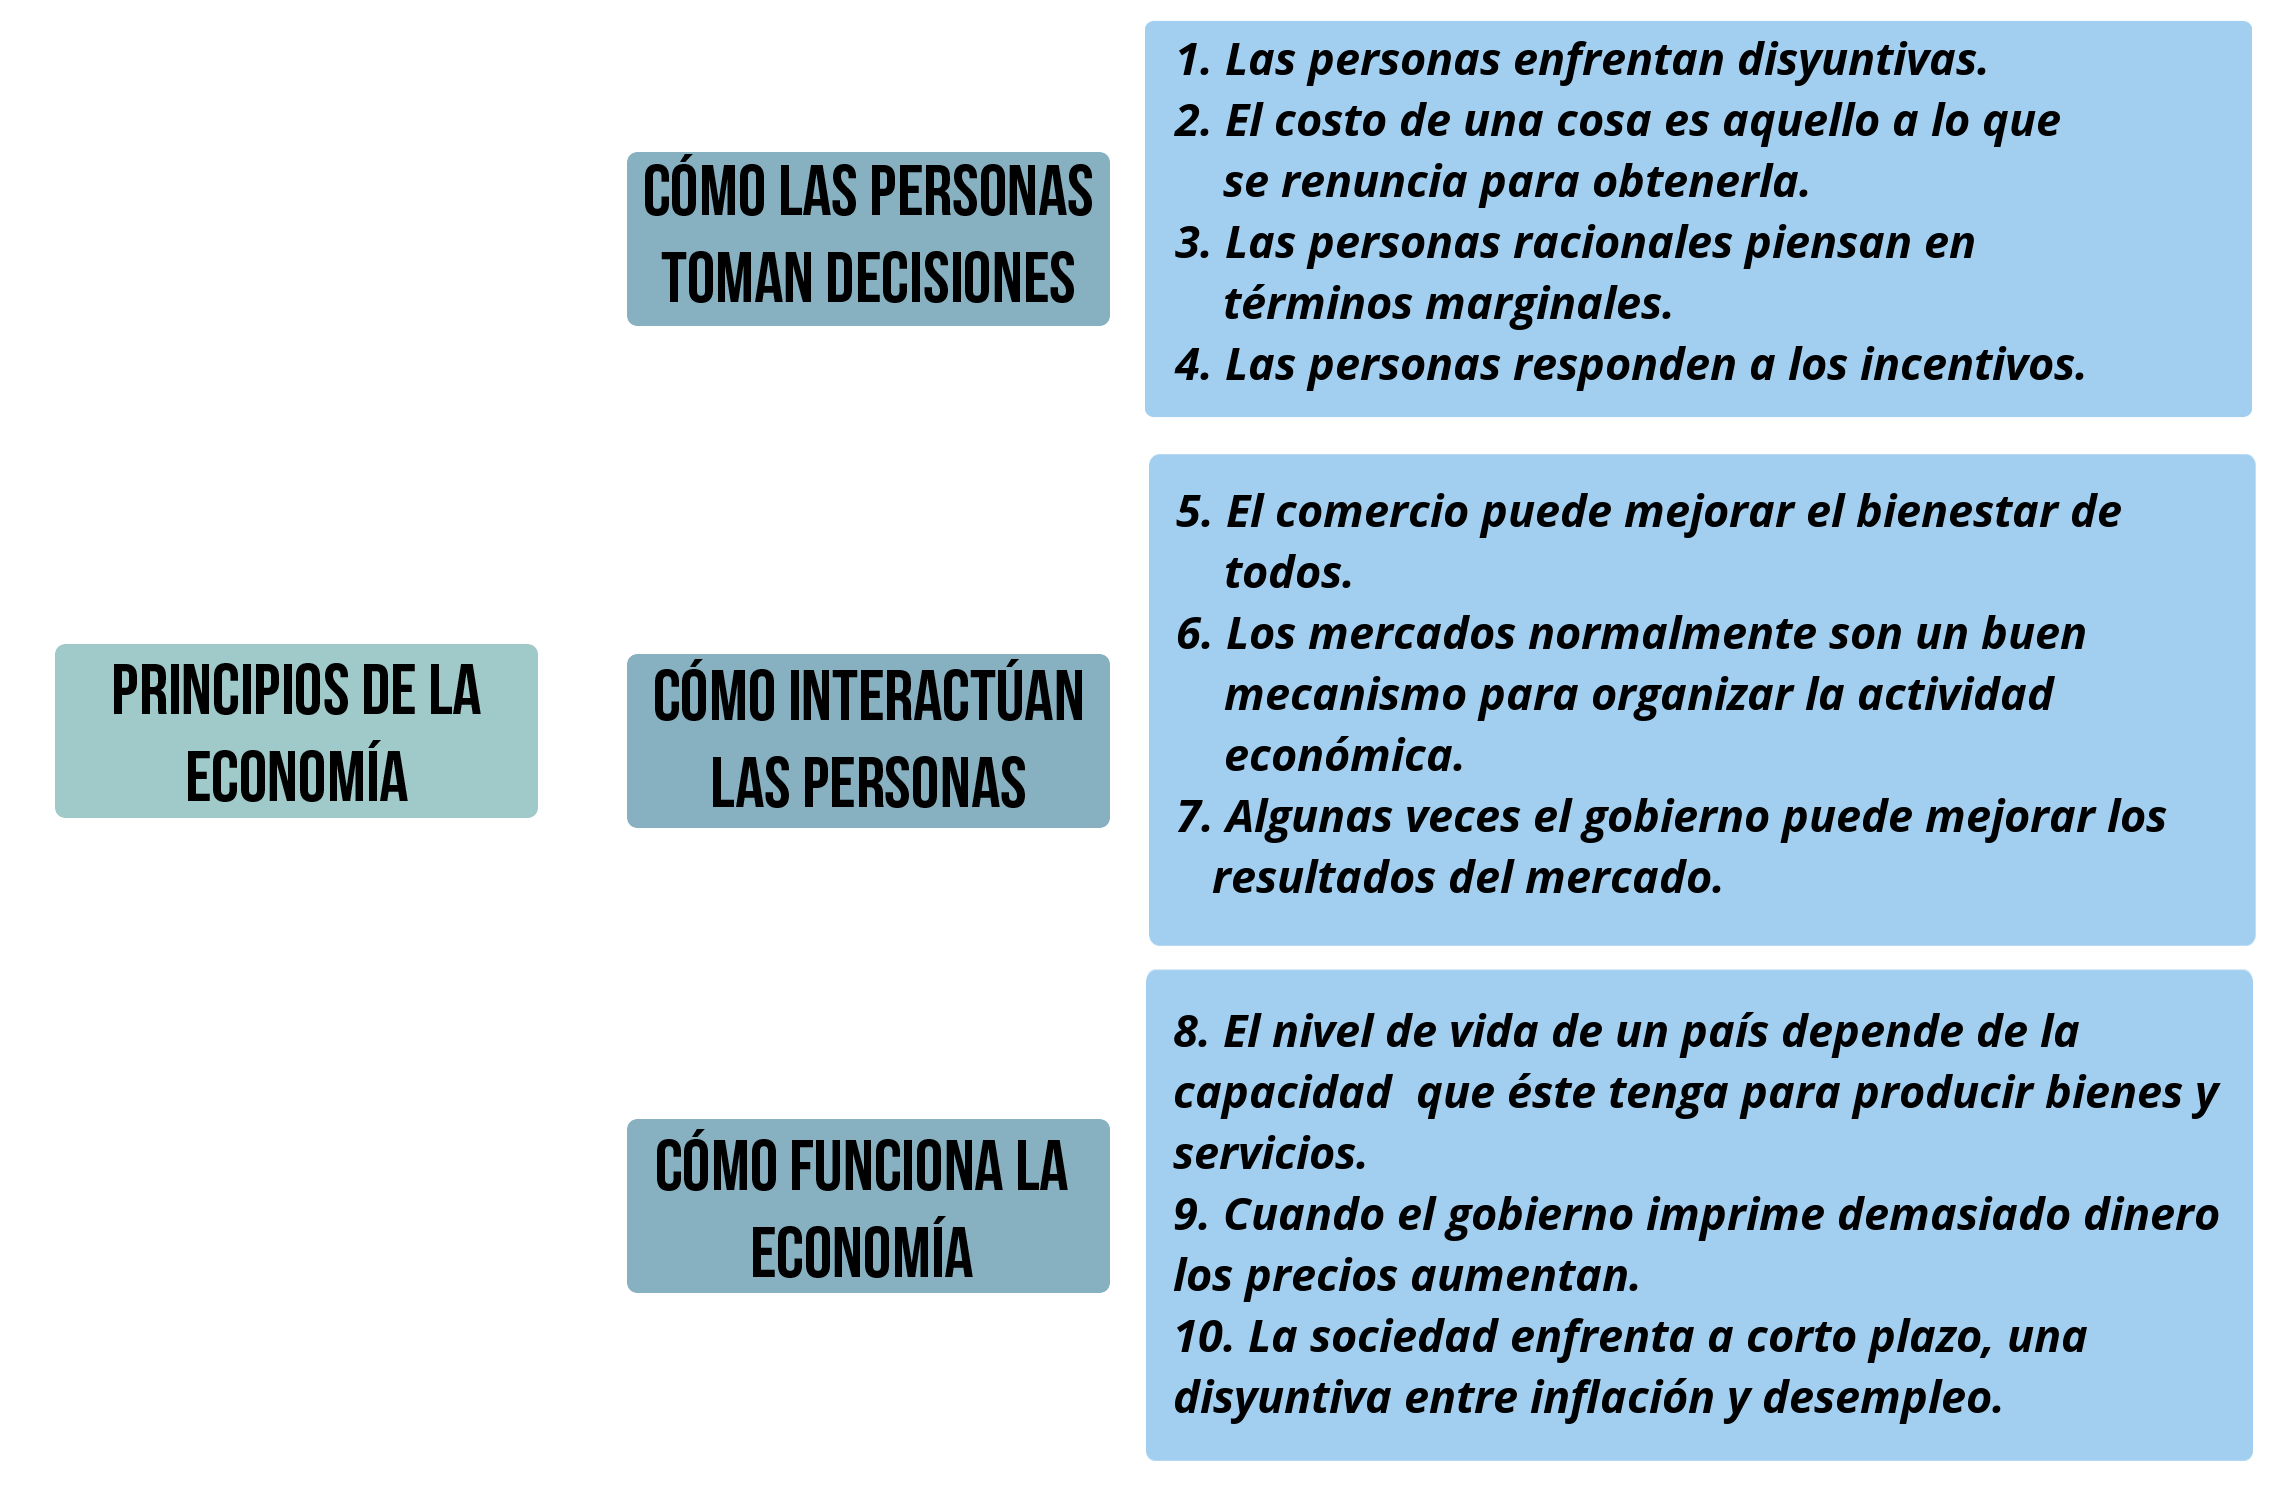
\includegraphics[width=0.65\linewidth]{images/PrincipiosEconomia}\\
\end{center}

\subsection{Cómo las personas toman decisiones.-}
Una economía no tiene nada de misterio. Independientemente de que nos refiramos
a la economía de Bolivia, a la de Estados Unidos o a la del mundo, \textbf{la economía
es solamente un grupo de personas interactuando en su vida diaria}. El comportamiento de una economía refleja el comportamiento de sus individuos, y es por esto que iniciamos el estudio de la economía con cuatro principios que regulan a los individuos al tomar decisiones.
\subsubsection{Principio 1: Las personas enfrentan disyuntivas.}
Quizá haya escuchado el dicho que asegura: \textit{"No se puede hablar y silbar al mismo tiempo".} Este dicho es muy cierto y resume la primera lección sobre toma de decisiones, \textcolor[rgb]{0,0,0.37}{ya que para obtener lo que queremos, en general tenemos que renunciar a algo que también nos gusta,} por tanto, \textcolor{azul1}{\textbf{tomar decisiones significa elegir entre dos objetivos.}} \\

La forma de actuar de la mayoría de personas implica tomar decisiones y establecer prioridades. Las disyuntivas están presentes en todos los ámbitos de la vida pero en las relaciones económicas adquieren una dimensión superior, marcando en última instancia la calidad de vida de las personas. Por ello, cualquier decisión debe tomarse ponderando si aquello que se consigue mejora aquello que se pierde o se deja de ganar.\\



Por ejemplo, si pensamos que un estudiante debe decidir cómo distribuir su recurso más valioso, es decir, su tiempo. El  estudiante puede pasar todo su tiempo estudiando matemáticas, física o dividiéndolo entre estas dos materias. Por cada hora que el estudiante destine a estudiar una materia, automáticamente dejará de estudiar la otra materia durante ese tiempo. Por cada hora que pase estudiando, automáticamente dejará de dedicar dicha hora a tomar una siesta, pasear en bicicleta, ver la
televisión o trabajar medio tiempo para así tener algo de dinero extra.\\

Ahora piense en los padres que deciden cómo gastar el ingreso familiar. Pueden comprar ropa, comida o salir de vacaciones; pueden también ahorrar una parte de su ingreso para cuando se jubilen; o bien, para pagar la educación de sus hijos. Cuando
los padres deciden gastar un dólar en uno de estos bienes, automáticamente tienen un dólar menos para gastar en otra cosa.\\

Como se expuso lineas arriba las personas toman decisiones cada día, pero también las sociedades, entendidas como el conjunto de personas, pueblos o naciones que conviven bajo normas comunes, enfrentan disyuntivas, por ejemplo una de las disyuntivas fundamentales que toda sociedad enfrenta esta dada entre la eficiencia y la equidad. La \textbf{eficiencia} significa que la sociedad extraer el máximo beneficio de sus recursos escasos. La \textbf{equidad} significa que la sociedad distribuye igualitariamente esos beneficios entre sus miembros. En otras palabras, piense en los recursos de la economía como un pastel que debe repartirse. La eficiencia sería el tamaño del pastel y la equidad la manera en cómo se reparte entre los diferentes individuos dicho pastel.\\





\subsubsection{Principio 2: El costo de una cosa es aquello a lo que se renuncia para obtenerla.}
\subsubsection{Principio 3: Las personas racionales piensan en términos marginales.}
\subsubsection{Principio 4: Las personas responden a incentivos.}

%-----------------------------------------------------------------------
% CAPITULO 2
%-----------------------------------------------------------------------
\chapter{VARIABLES SOCIOECONÓMICAS} 
\section{Introducci�n.}
Los mercados hacen bien muchas cosas, pero no lo hacen todo bien, es as� que en una econom�a de mercado, la interacci�n de la oferta y demanda es la que determina la cantidad y precio de equilibrio de los bienes y servicios transados. Asimismo, el mercado se encarga de la distribuci�n de la renta a trav�s de la posesi�n de los factores productivos (capital, trabajo, etc.) \\

Pero la competencia perfecta y las excelencias derivadas de este mercado como su pretendida eficiencia econ�mica s�lo se dan cuando se cumplen un conjunto de condiciones muy restrictivas que podemos calificar como de ideales, es decir, que la existencia de mercados 100\% eficientes es una construcci�n te�rica que permite analizar los modelos econ�micos pero que dif�cilmente se da en la vida real debido a la existencia de algunos \textbf{fallos del mercado.}\\

Conocemos, por los \textit{"principios de la econom�a"} estudiados en el capitulo I, que \textit{"los mercados normalmente son un buen mecanismos para organizar la actividad econ�mica"} (6� principio.) pero tambi�n sabemos que \textit{"el gobierno puede mejorar en algunas ocasiones los resultados del mercado" (8� principio).} Es as� que ante la existencia de estos fallos del mercado es conveniente la intervenci�n del gobierno a trav�s de pol�ticas gubernamentales espec�ficas.\\

Una econom�a de mercado no siempre puede garantizar la distribuci�n equitativa de los beneficios de la prosperidad econ�mica, y ante un escenario que presenta inequidades, la intervenci�n del gobierno se constituye en un mecanismo que permite lograr una distribuci�n m�s equitativa del bienestar econ�mico, pero para que el gobierno desarrolle determinadas acciones o pol�ticas es fundamental conocer la realidad donde se va intervenir y esto se logra a trav�s del manejo y conocimientos de las variables econ�micas y sociales de un determinado territorio.   
\begin{scaja}
	\paragraph{�Por qu� el Gobierno interviene la econom�a?}
	Una de las razones por las cuales necesitamos al gobierno es porque las econom�as de mercado necesitan instituciones que hagan
	valer los derechos de propiedad de las personas para que �stas puedan ejercer propiedad y control sobre los recursos escasos. Pero tambi�n necesitamos al gobierno para promover la eficiencia y la equidad en la econom�a ya que la mayor�a de las medidas econ�micas aspiran a generar mayor crecimiento econ�mico y mayor bienestar a trav�s de una mejor redistribuci�n de la riqueza.
\end{scaja}

\begin{definicion}[\textcolor[rgb]{0,0,0.55}{Fallos del mercado:}]
{\small 	Es una situaci�n que se produce cuando el mercado, por si s�lo, no es capaz de asignar los recursos de forma eficiente.}
\end{definicion}

\begin{definicion}[\textcolor[rgb]{0,0,0.55}{Estado:}]
	{\small Forma de organizaci�n pol�tica, dotada de poder soberano e independiente, que integra la poblaci�n e instituciones de un territorio.}
\end{definicion}

\begin{definicion}[\textcolor[rgb]{0,0,0.55}{Gobierno:}]
	{\small �rgano superior del poder ejecutivo de un Estado o de una comunidad pol�tica, por tanto, son las autoridades que dirigen, controlan y administran las instituciones del Estado.}
\end{definicion}

\subsection{{\large Los fallos de mercado.}}
La existencia de fallos de mercado se puede deber a la presencia de alguno de los tres hechos siguientes: \textbf{competencia imperfecta, externalidades e informaci�n imperfecta.}\\

\subsubsection{\textcolor[rgb]{0,0,0.55}{\underline{{\normalsize Competencia Imperfecta:}}}}
Una posible causa de una falla de mercado se relaciona con el \textbf{poder de mercado} que tienen las empresas, esto es,
capacidad para influir sobre los precios que tiene y como a trav�s de este poder se impide que exista un mercado eficiente en la econom�a.\\

El poder de mercado deriva en mercados no competitivos, entendido como son aquellos mercados en los que el productor o productores son lo suficientemente grandes como para tener un efecto notable sobre el precio. En los mercados de competencia imperfecta, el precio no se acepta como un dato ajeno, sino que los oferentes intervienen activamente en su determinaci�n.\\

Las causas de imperfecci�n en los mercados son los factores que suele impedir que se incorporen un mayor n�mero de empresas en un mercado determinado y estas causas son principalmente dos:
\begin{itemize}
	\item Los costos de producci�n.
	\item Las barreras a la entrada de nuevos competidores en una industria 
\end{itemize}

\paragraph{{\normalsize Costos de Producci�n.}}
La estructura de costos y el nivel tecnol�gico son los factores determinantes del n�mero de empresas que puede soportar una
industria o un mercado espec�fico y las dimensiones que �stas pueden tener, por tanto, aquellos que puedan producir bienes y servicios a un menor costo tienen mayores posibilidades de incrementar su poder de mercado y por medio de estos limitar la cantidad de nuevos oferentes en una determinada industria o mercado. 

\begin{definicion}[\textcolor[rgb]{0,0,0.55}{Costos de Producci�n:}]
	Es el conjunto de gastos que son necesarios para producir bienes o servicios
\end{definicion}

\paragraph{{\normalsize Barreras de Entrada.}}
Las barreras de entrada a un mercado son obst�culos de diversos tipos que complican o dificultan el ingreso a un mercado de empresas, marcas o productos nuevos. Estas barreras representan un aspecto fundamental en la determinaci�n de la estructura del mercado, ya que afectan sustancialmente el n�mero de empresas, la concentraci�n, la amenaza de entrada y el nivel de competencia de una industria. \\

Las principales barreras de entrada que enfrenta un potencia competidor las podemos clasificar en tres categor�as: las restricciones legales, restricciones naturales y restricciones estrat�gicas.

\begin{itemize}
	\item \textbf{Barreras Legales:} Tienen su origen en la normativa y corresponden a aqu�llas con las cuales, por alg�n cuerpo legal, se impide, o al menos se encarece, la entrada de nuevas empresas en una industria.
	\item \textbf{Barreras Econ�micas:} Est�n ligadas a la inversi�n necesaria para la entrada en el mercado de nuevos competidores, por ejemplo el gasto en publicidad enfocada a dar a conocer la nueva empresa y sus productos o la parte de inversi�n dedicada al desarrollo y la innovaci�n tecnol�gica necesarios en gran n�mero de sectores que permitan superar las barreras econ�micas ligadas a costos, precios o diferenciaci�n de productos; Entre las principales barreras econ�micas podemos mencionar:
	\begin{itemize}
		\item \textbf{Econom�as a escala:} que relaciona los costos con la producci�n, existe econom�a de escala cuando el costo medio decrece con el nivel de producci�n. Es decir, cada unidad adicional que produce la empresa (constituida en determinado mercado) disminuye su costo unitario. 
		\item \textbf{Diferenciaci�n de producto:} la diferenciaci�n ocurre cuando las empresas ya establecidas tienen prestigio de marca o una cartera de clientes establecida.
		\item \textbf{Los precios:} Se pueden constituir en una barrera de entrada, si pensamos que 
		el caso de 	una empresa establecida fija los precios lo suficientemente bajos de manera que los potenciales entrantes
		se sientan desalentados de ingresar a la industria o mercado espec�fico.
	\end{itemize}

Estas barreras de entrada, entendidas como los factores que limitan la entrada de nuevas empresas en una industria, de forma que, cuando las barreras de entrada son altas, la industria tendr� pocas empresas y escasas presiones para competir.  

\end{itemize}

\paragraph{{\normalsize Mercados de Competencia Imperfecta.}}
En funci�n del n�mero, del tama�o de los oferentes, del grado de concentraci�n entre las empresas concurrentes y de la homogeneidad o heterogeneidad de los productos, podemos clasificar  los mercados de competencia imperfecta en tres categor�as diferentes:
\begin{itemize}
	\item \textbf{El monopolio:} es el caso extremo de la competencia	imperfecta y se caracteriza porque hay un �nico vendedor
	que controla la industria.
	\item \textbf{El oligopolio:} este mercado se caracteriza porque hay pocos vendedores, de forma que cada empresa 
	puede influir en el precio de mercado y en la conducta 	de sus competidores.\\
\end{itemize}

\subsubsection{\textcolor[rgb]{0,0,0.55}{\underline{{\normalsize Externalidades:}}}}

Las externalidades se definen como decisiones de consumo, producci�n e inversi�n que toman los individuos, los hogares y las empresas y que afectan a terceros que no participan directamente los procesos antes referidos. Una externalidad surge cuando una persona se dedica a una actividad que influye en el bienestar de un tercero al que no se le paga ni se le compensa por dicho efecto.\\

Ante la presencia de externalidades, el intere?s de la sociedad en el resultado del mercado va ma?s alla? del bienestar de los compradores y vendedores que participan en el mercado, por tanto, la inclusi�n del bienestar de terceros que resultan afectados directa o indirectamente es por las acciones de compradores o vendedores es de mayor que el bienestar de estos �ltimo.\\

Si el impacto sobre el tercero es negativo, se conoce como externalidad negativa. Si le beneficia, se llama externalidad positiva:

\begin{itemize}
	\item     \textbf{Externalidad negativa:} Surge cuando no se asumen todos los costos de un efecto negativo. Hablamos de externalidades negativas cuando, por ejemplo, una empresa contamina su entorno o cuando una persona arroja basura a la calle. En estos dos casos, se genera un costo social, ya que es toda la sociedad por igual la que sufre las consecuencias de sus acciones y el precio de mercado no recoge este costo.
	\item \textbf{Externalidad positiva:} Surge de un efecto positivo que no se reporta como beneficio. Un ejemplo de externalidad positiva que podemos mencionar es la investigaci�n cient�fica, de la cual se beneficia la sociedad en general. Otro ejemplo ser�a la utilizaci�n de energ�as renovables, del que se beneficia la sociedad porque la persona o empresa que las utiliza no est� contaminando. En estos casos, los precios de mercado no recogen los beneficios reales.
\end{itemize}

Entonces, cuando una \textbf{acci�n privada} tiene efectos colaterales o externos que afectan a otras personas de manera importante existe un problema de externalidades. Estos efectos externos crean una divergencia entre los costos y valoraciones privadas y sociales. Dado que los efectos externos no se reflejan en los precios de mercado, �stos facilitan informaciones que impiden alcanzar la eficiencia econ�mica.

\begin{figure}[h]
	\centering
	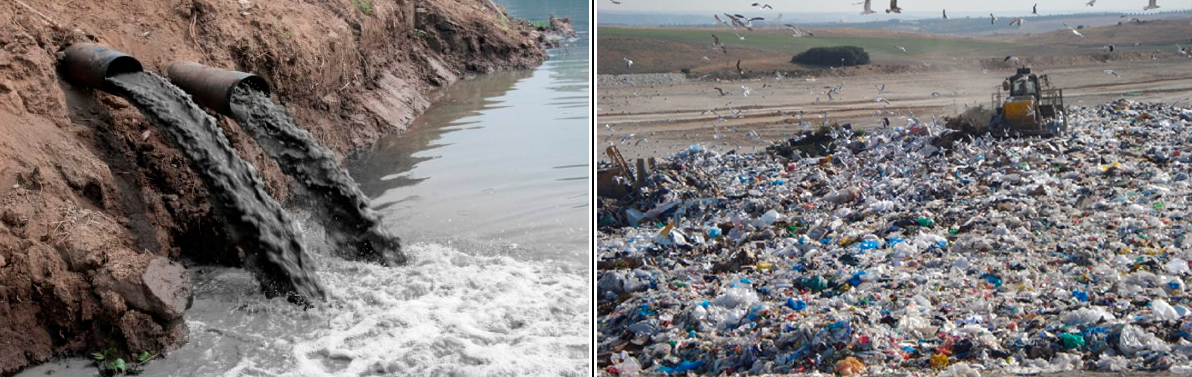
\includegraphics[width=0.7\linewidth]{images/contamina}
	\caption[Externalidades Negativas]{La contaminaci�n como externalidad negativa (efecto de la producci�n y el consumo)}
	\label{fig:contamina}
\end{figure}

Buena parte de las externalidades negativas se deben a la contaminaci�n. Las ciudades contaminan los r�os, los lagos y los mares con sus vertidos y las empresas con los suyos. Los autom�viles, las calefacciones y las industrias contaminan la atm�sfera. Estas externalidades crean ineficiencias.

\begin{definicion}[\textcolor[rgb]{0,0,0.55}{Externalidad}]
	El efecto no compensado de las acciones de una persona sobre el bienestar de un tercero.
\end{definicion}

\begin{ejemplos}
	Las externalidades se presentan en diferentes formas, al igual que las pol�ticas que se formulan para corregir las fallas del mercado. He aqu� algunos ejemplos:
	\begin{ejemplo}
		El tubo de escape de los autom�viles es una externalidad negativa porque genera smog que otras personas tienen que respirar. Como resultado de esta externalidad, los conductores tienden a contaminar demasiado. El gobierno trata de resolver este problema estableciendo normas para las emisiones de los automo?viles, tambie?n podrian aplicar un impuestos a la gasolina para reducir la cantidad de personas que conducen vehi?culos automotores.
	\end{ejemplo}
	\begin{ejemplo}
	Los edificios hist�ricos restaurados constituyen una externalidad positiva, porque las personas que pasan por donde se encuentran disfrutan de su belleza y el recuerdo de la historia que evocan. Los propietarios de los edificios no obtienen el beneficio total de la restauraci�n y, en consecuencia, tienden a deshacerse muy r�pido de los edificios viejos. Muchos gobiernos locales responden a este problema regulando la destrucci�n de edificios histo?ricos y ofreciendo exenciones de impuestos a los propietarios que los restauran.
    \end{ejemplo}

	\begin{ejemplo}
	Los perros que ladran crean una externalidad negativa, porque el ruido molesta a los vecinos. Los due�os de los perros no cubren el costo total del ruido y, por tanto, tienden a tomar pocas medidas precautorias que impidan que sus perros ladren. Para resolver este problema los gobiernos locales proh�ben "alterar el orden pu?blico".
	\end{ejemplo}

	\begin{ejemplo}
	La investigacio�n de nuevas tecnologi?as es una externalidad positiva porque crea conocimiento que otras personas pueden utilizar. Debido a que los investigadores no pueden captar los beneficios completos de sus inventos, tienden a destinar pocos recursos a la investigacio?n.
	\end{ejemplo}
En cada uno de estos casos, alg�n tomador de decisiones no considera los efectos externos de su comportamiento. En respuesta, el gobierno trata de influir en su comportamiento para proteger los intereses de terceros.
\end{ejemplos}

\paragraph{{\normalsize Instrumentos del Estado para combatir las externalidades.}}
Debido a que compradores y vendedores desatienden los efectos externos de sus acciones cuando deciden cu�nto demandar u ofrecer, por tanto, el equilibrio del mercado no es eficiente cuando se presentan externalidades, es decir, el equilibrio es incapaz de maximizar el beneficio total para la sociedad.\\

Para luchar contra la ineficiencia derivada de las externalidades, los Estados suelen establecer "regulaciones sociales" a trav�s de \textbf{controles directos}, o bien recurrir a \textbf{incentivos econ�micos}, es decir, "medidas basadas en el mercado".
\begin{itemize}
	\item \textbf{Regulaciones Sociales:} Para dar soluci�n a una externalidad, el gobierno puede exigir o prohibir ciertas conductas mediante la aplicaci�n de \textbf{\textcolor[rgb]{0,0.24,0.5}{"Controles Directos."}} Por ejemplo, es un delito verter sustancias qu�micas venenosas en el sistema de abastecimiento de agua. En este caso, los costos externos para la sociedad exceden	por mucho los beneficios para el que contamina. Por tanto, el gobierno instituye una	pol�tica de orden y control que proh�be este tipo de actos.\\
	
	Los controles directos se constituyen en detalladas instrucciones sobre las acciones a tomar, la tecnolog�a que se debe utilizar para controlar la contaminaci�n y d�nde se debe aplicar. Las leyes y normas o regulaciones ambientales son tipos de controles que establecen los gobiernos prohibiendo determinadas acciones o estableciendo procedimientos para minimizar los efectos negativos derivados de las actividades comerciales o de consumo, adem�s de estipular las penalizaciones a pagar por los da�os causados a otras personas.\\
	
	Pero este tipo de controles directos no dejan margen para aplicar nuevos m�todos que permitan combatir las externalidades y la experiencia nos muestran que los resultados de la aplicaci�n de dichos controles sueles se costos y derivan en la vulneraci�n de las mismas.
	
	\item \textbf{Medidas Basadas en el Mercado:} Un segundo tipo de instrumentos para combatir la ineficiencia	provocada por las externalidades, y en particular la contaminaci�n, son los que recurren a \textbf{\textcolor[rgb]{0,0.24,0.5}{"incentivos econ�micos"}} que proporciona el mercado. En este sentido son dos los tipos de soluciones empleadas: \textbf{los impuestos sobre emisiones} y los \textbf{permisos transferibles de contaminaci�n.}\\
	
	\textbf{\textcolor[rgb]{0,0.24,0.5}{Impuesto sobre emisiones:}} Son un tipo de \textbf{impuesto correctivo} que tiene el prop�sito de inducir a los sujetos responsables de la externalidad ha tomar en cuenta el costo social que surge de una determinada actividad desarrollada por estos, es as� que los impuestos sobre las emisiones obligan, por ejemplo, a las empresas a pagar un impuesto sobre su contaminaci�n igual a la cantidad de da�os externos ocasionados.\\
	
	En esencia, este tipo de impuestos asigna un precio al derecho a contaminar, por tanto, pretende internalizar la externalidad forzando a los sujetos contaminantes pague los costos sociales de sus actividades (producci�n y/o consumo).\\
	
	\textbf{\textcolor[rgb]{0,0.24,0.5}{Permisos transferibles para contaminar:}} Cuando se recurre a este m�todo, en vez de obligarle a la empresa contaminante a pagar una determinada cantidad por unidad de contaminaci�n y permitirle elegir el nivel de contaminaci�n, las autoridades eligen el nivel o umbral m�ximo de contaminaci�n total y determinan el n�mero adecuado de permisos.\\
	
	Este m�todo de actuar permite que las empresas contaminantes que pueden reducir sus emisiones de forma m�s barata lo hagan y vendan sus permisos a las	que necesitan m�s permisos para nuevas plantas o porque	no tienen mucho margen para reducir las emisiones y les	resulta m�s conveniente comprar permisos en lugar de instalar unos equipos caros contra la contaminaci�n.\\
	
\end{itemize}


\subsubsection{\textcolor[rgb]{0,0,0.55}{\underline{{\normalsize Informaci�n Incompleta:}}}}
El tercer tipo de fallo del mercado, junto a la competencia
imperfecta y las externalidades, es la \textbf{informaci�n imperfecta.} La teor�a de libre mercado supone que los compradores y los vendedores tienen total informaci�n sobre
los bienes y los servicios que compran y venden. Se supone que las empresas conocen perfectamente todos los aspectos t�cnicos necesarios para producir en su industria y que los consumidores conocen la calidad y los precios de los bienes que consumen. Por ejemplo, se supone que los consumidores saben qu� autom�viles se encuentran en buen estado y cuales no o cu�l es la seguridad y la eficacia de los f�rmacos que toman. \\

La realidad es muy distinta de este mundo idealizado y lo relevante es saber en qu� medida son perjudiciales las desviaciones respecto de la informaci�n perfecta. En algunos casos, la p�rdida de eficiencia es escasa. As�, por ejemplo, apenas resultaremos perjudicados si compramos una pizza con una masa distinta de la de otra. En otros casos, la p�rdida es grave. Entonces, \textit{los mercados normalmente suministran a los consumidores o a los productores una informaci�n imperfecta para la toma de decisiones.}\\

La realidad es muy distinta de este mundo idealizado ya que la informaci�n asim�trica es caracter�stica de muchas situaciones de la vida real. A menudo el vendedor de un producto conoce su calidad mejor que el comprador. Normalmente los trabajadores conocen sus propias cualificaciones y capacidades mejor que los empresarios, los directivos conocen mejor los costes de la empresa, la posici�n competitiva y las oportunidades de inversi�n que los propietarios o accionistas y los m�dicos suelen tener m�s informaci�n sobre las enfermedades que los pacientes.\\

Para analizar las implicaciones de la existencia de informaci�n imperfecta, empecemos por considerar qu� ocurre cuando algunos tienen m�s informaci�n que otros, es decir, cuando hay \textbf{informaci�n asim�trica}, existir� \textcolor[rgb]{0,0.18,0.39}{informaci�n asim�trica cuando la informaci�n sobre la calidad y caracter�sticas de los bienes y servicios intercambiados o sobre las acciones o caracter�sticas de los agentes que influyen en aqu�llas no est� distribuida de forma sim�trica entre los consumidores y los productores,} por tanto, la existencia asimetr�as de informaci�n puede afectar el nivel de precios en los mercados como consecuencia del uso indebido de la informaci�n privilegiada.\\

\subsection{{\large Las Funciones del Estado.}}

Tal como hemos se�alado, las econom�as de mercado tienen imperfecciones que generan
males como la contaminaci�n excesiva, el desempleo y diferencias de renta y riqueza que se consideran �ticamente rechazables. Esto significa que las econom�as de mercado no se
ajustan totalmente al mundo idealizado de la mano invisible que funciona armoniosamente. Por estas razones, el Estado asume muchas tareas que tratan de paliar los fallos
del mecanismo del mercado.\\

El Estado interviene en la actividad econ�mica procurando la eficiencia, la equidad, la estabilidad econ�mica y el crecimiento y el bienestar. Este conjunto de actividades del Estado se engloban en tres grandes funciones que son:\\
\begin{itemize}
	\item Mejorar la eficiencia econ�mica combatiendo los
	fallos del mercado.
	\item Estabilizar la econom�a y propiciar el crecimiento
	econ�mico, mediante la pol�tica econ�mica.
	\item Procurar la equidad mejorando la distribuci�n de la
	renta.
\end{itemize}
El Estado contribuye a la asignaci�n socialmente deseable de los recursos. En este sentido, el Estado interviene tratando de contribuir a corregir los fallos del
mercado analizados previamente (competencia imperfecta, las externalidades y la informaci�n imperfecta). En este sentido, el Estado interviene tratando de limitar el poder
de mercado de las empresas monopol�sticas u oligopol�sticas, luchando contra los efectos nocivos de las externalidades, especialmente la contaminaci�n, proveyendo bienes p�blicos y tratando de suministrar informaci�n a los consumidores para que tomen decisiones
bien documentadas y as� paliar los efectos de la informaci�n imperfecta.\\

\subsubsection{El Estado y la Actividad Econ�mica:}

El Estado en la b�squeda de sus objetivos recurre a diferentes instrumentos que le permita cumplir sus funciones, es as� que la Pol�tica Fiscal y la Pol�tica Monetaria son los principales instrumentos del Estado para intervenir en la actividad econ�mica.\\

	\textbf{\textcolor[rgb]{0,0.24,0.5}{Pol�tica Fiscal:}}	\small Se entiende por pol�tica fiscal al \textbf{conjunto de medidas relativas al r�gimen tributario, gasto publico, endeudamiento interno externo del Estado, y a las operaciones y situaci�n financiera de las entidades y organismos aut�nomos. } \\
	
	\textbf{\textcolor[rgb]{0,0.24,0.5}{Pol�tica Monetaria:}} \small Es el conjunto de acciones llevadas por el \textbf{Banco Central}, \textbf{cuyo fin es influir en el crecimiento econ�mico mediante manejo de variables monetarias de la econom�a.} Variables como la inflaci�n, emisi�n monetaria, funcionamiento del banco Central, regulaci�n de bancos comerciales, tipo de inter�s, protecci�n a reservas de oro y d�lares.\\
	
	La pol�tica fiscal y monetaria tiene un abanico de instrumentos, pero son tres los instrumentos b�sicos que utiliza el Estado para influir en la actividad econ�mica: los \textbf{impuestos}, los	\textbf{gastos} y la \textbf{regulaci�n}.\\
	
	\begin{cajaejercicios1}[Impuestos]
		Los impuestos son un pago al Estado, y estos reducen la renta privada y el gasto privado y son fuente de recursos para el gasto p�blico. \\
		
		El conjunto impuestos, esto es, el sistema tributario,	tambi�n sirve para reducir los incentivos para llevar a cabo determinadas actividades sujetas a impuestos,
		como contaminar o fumar, y fomentar otras que est�n	menos gravadas, como es comprar una vivienda, estudiar	o investigar, etc.\\
				
		Cuando el Estado establece los impuestos est� decidiendo la manera en que van a obtenerse los recursos necesarios de los hogares y de las empresas para darle un fin p�blico, es decir, el Estado para hacer frente a los gastos p�blicos, esto es, a todos	los programas, proyectos y actividades llevadas a cabo por el mismo,
		el Estado establece una serie de impuestos y lo que falta lo obtiene mediante cr�dito.\\
		
	\end{cajaejercicios1}

	\begin{cajaejercicios1}[Gastos]
		El gasto p�blico es la cantidad de recursos financieros, materiales y humanos que el sector p�blico representado por el gobierno emplea para el cumplimiento de sus funciones, este conjunto de erogaciones que realiza el Estado esta orientado a la producci�n bienes y servicios p�blicos en un periodo determinado.\\
		
		El gasto p�blico comprende desde las compras de bienes	y servicios por parte del sector p�blico a los sueldos de los	funcionarios p�blicos, la Seguridad Social y otras transferencias, y los intereses. De igual forma las inversiones p�blicas forman parte del gasto p�blico total reflejados en programas y proyectos de inversi�n p�blica.\\
		
		Desde la perspectiva de gesti�n del gasto p�blico se pueden identificar tres objetivos principales:
		\begin{itemize}
			\item Lograr estabilidad econ�mica y la disciplina fiscal.
			\item Alcanzar una adecuada distribuci�n social de los recursos.
			\item Promover la eficiencia a trav�s de gasto p�blico, mediante la correcci�n de fallas de mercado
		\end{itemize}
	\end{cajaejercicios1}
	Estos objetivos tienen la finalidad de generar mayores niveles de crecimiento y desarrollo econ�mico y por medio de estos bienestar para su poblaci�n.\\
	
	\begin{cajaejercicios1}[Regulaci�n]
		La regulaci�n, es el control por parte del Estado de la actividad econ�mica, estas regulaciones lleva a los individuos y empresas a realizar determinadas actividades o abstenerse de realizarlas.\\
		
		Desde una perspectiva general la regulaci�n es de dos tipos: econ�mica y social. 
		\begin{itemize}
			\item La \textbf{regulaci�n econ�mica} se refiere al control de los precios, la producci�n, las condiciones de entrada y salida del mercado y la calidad de los	productos y servicios de una determinada industria.\\
			
			\begin{definicion}[\textcolor[rgb]{0,0,0.55}{Regulaci�n Econ�mica:}]
				La regulaci�n econ�mica consiste en las normas destinadas a controlar las decisiones de las empresas relacionadas con los precios, las ventas
				o la producci�n.
			\end{definicion}

			
			\item La \textbf{regulaci�n social} es la que se emplea para proteger
			el medio ambiente, la salud y la seguridad de los trabaja-
			dores y de los consumidores, y se encamina a tratar de
			corregir los efectos secundarios o externalidades de la
			actividad econ�mica.
			 
		\end{itemize}
	\end{cajaejercicios1}
\subsection{{\large Variables Socioecon�micas.}}
Si la finalidad del Gasto P�blico, como pol�tica fiscal, es el de generar mayores niveles de crecimiento y desarrollo econ�mico y por medio de estos bienestar para su poblaci�n, es importante poder precisar que debemos entender por Crecimiento, Desarrollo o Subdesarrollo y Bienestar y como el analizar estas condiciones a trav�s de variables socioecon�micas permitir�n desarrollar diagn�sticos mas precisos y orientar las decisiones de gasto p�blico.\\

% Define box and box title style
\tikzstyle{mybox} = [draw=azul1!90, fill=yellow!15, very thick,
rectangle, rounded corners, inner sep=10pt, inner ysep=10pt]
\tikzstyle{fancytitle} =[fill=azul1!90, text=white]

\begin{tikzpicture}
\node [mybox] (box){%
	\begin{minipage}{0.95\textwidth}
	El crecimiento econ�mico es definido como la capacidad de una econom�a para producir cada vez m�s bienes y servicios, por tanto, es el aumento del producto e ingreso.
	\end{minipage}
};
\node[fancytitle, right=10pt] at (box.north west) {\textbf{Crecimiento Econ�mico}};
%\node[fancytitle, rounded corners] at (box.east) {$\clubsuit$};
\end{tikzpicture}
\\
%%%%%%%%%%%%%%%%%%%%%%%%%%%%%%%%%%%%

\tikzstyle{mybox} = [draw=miverde, fill=yellow!15, very thick,
rectangle, rounded corners, inner sep=10pt, inner ysep=10pt]
\tikzstyle{fancytitle} =[fill=miverde, text=white]

\begin{tikzpicture}
\node [mybox] (box){%
	\begin{minipage}{0.95\textwidth}
	El desarrollo econ�mico puede definirse gen�ricamente como crecimiento
	sostenible desde tres puntos de vista: econ�mico, social y medioambiental,
	por tanto, una mejora en el desarrollo econ�mico se ve reflejado en el
	incremento del bienestar material de la poblaci�n.
	\end{minipage}
};
\node[fancytitle, right=10pt] at (box.north west) {\textbf{Desarrollo Econ�mico}};
%\node[fancytitle, rounded corners] at (box.east) {$\clubsuit$};
\end{tikzpicture}
\\
%%%%%%%%%%%%%%%%%%%%%%%%%%%%%%%%%%%%

\tikzstyle{mybox} = [draw=rojo1, fill=yellow!15, very thick,
rectangle, rounded corners, inner sep=10pt, inner ysep=10pt]
\tikzstyle{fancytitle} =[fill=rojo1, text=white]

\begin{tikzpicture}
\node [mybox] (box){%
	\begin{minipage}{0.95\textwidth}
	Es la situaci�n de un pa�s o regi�n que no alcanza determinados niveles de crecimiento econ�micos, sociales y mediambientales.
	\end{minipage}
};
\node[fancytitle, right=10pt] at (box.north west) {\textbf{Subdesarrollo}};
%\node[fancytitle, rounded corners] at (box.east) {$\clubsuit$};
\end{tikzpicture}

\begin{scaja}
		\textbf{El subdesarrollo es una estructura productiva atrasada en comparaci�n con otros pa�ses}, las condiciones de vida de la poblaci�n son limitadas, se tiene dependencia con el mercado internacional, 	desigualdad econ�mica, no se tienen bienes de capital para la inversi�n en rubros necesarios para	el pa�s, los sectores industriales son insuficientes o atrasados, hay baja productividad, bajos salarios y 	competencia con productos importados, entre otros factores.
\end{scaja}

Si las condiciones de vida de la poblaci�n son limitada, es obligaci�n del gobierno de dirigir sus esfuerzos de pol�tica econ�mica a generar las condiciones de desarrollo, por tanto de bienestar para su poblaci�n, pero la pregunta que surge ante esta situaci�n es: \textbf{�C�mo podemos medir el nivel de desarrollo de un pa�s, regi�n o localidad?}, y as� enfocar los esfuerzo en las situaciones m�s problem�ticas.\\

Una aproximaci�n a la caracterizaci�n del mundo desarrollado y subdesarrollado
o en v�as de desarrollo se puede obtener analizando los indicadores
socioecon�micos (\textcolor[rgb]{0,0.25,0.25}{variables socioecon�micas}) y comparando sus diferentes valores.
\\
%%%%%%%%%%%%%%%%%%%%%%%%%%%%%%%%%%%%

\tikzstyle{mybox} = [draw=rojo1, fill=red!15, very thick,
rectangle, rounded corners, inner sep=10pt, inner ysep=10pt]
\tikzstyle{fancytitle} =[fill=rojo1, text=white]

\begin{tikzpicture}
\node [mybox] (box){%
	\begin{minipage}{0.95\textwidth}
	De igual forma, si como estudiantes o el su futuro campo laboral, deben desarrollar proyectos de grado o proyectos de inversi�n, estos deben contar con un diagnostico base, que supone entre otras tareas, analizar las variables socioecon�micas m�s relevantes de acuerdo a la naturaleza del trabajo de investigaci�n.
	\end{minipage}
};
%\node[fancytitle, right=10pt] at (box.north west) {\textbf{Subdesarrollo}};
%\node[fancytitle, rounded corners] at (box.east) {$\clubsuit$};
\end{tikzpicture}


%\subsection{{\large Los .}}




%-----------------------------------------------------------------------
% CAPITULO 3
%-----------------------------------------------------------------------
\chapter{GEOGRAFÍA ECONÓMICA}
\section{Geografía:}
Etimológicamente, geografía significa \textbf{"descripción de la tierra"}. \\ 

La geografía estudia la descripción y disposición de los elementos en la superficie terrestre, por tanto, estudia el \textbf{espacio geográfico}, entendido como la resultante de las relaciones que la sociedad establece con la Tierra que habita.\\

Una Geografía que entiende el espacio geográfico como la expresión de las relaciones que las sociedades humanas establecen a lo largo del tiempo con los distintos ámbitos del planeta que habitan. Planeta que es, a la vez, su lugar de residencia, su fuente de vida y tal vez debamos decir también su prisión.\\ 

Sintéticamente podemos decir que el espacio geográfico, objeto de estudio de la Geografía, es Naturaleza modificada por la sociedad. En consecuencia, el espacio geográfico es una construcción social y la Geografía que lo estudia, una ciencia social.

\begin{scaja}
En sentido amplio, la geografía es la ciencia que estudia la superficie terrestre, las sociedades que la habitan y los territorios, paisajes, lugares o regiones que la forman al relacionarse entre si.	
\end{scaja}



El objetivo central de la geografía es conocer, comprender, explicar y analizar la relación que existe entre el ser humano y su medio.\\

El estudio geográfico comprende, en su estudio, tanto el medio físico como la relación de los seres humanos con este medio físico, por tanto busca las causas de los fenómenos geográficos y para ello se basa en tres principios:\\
\begin{itemize}
	\item \textbf{Principio de Causalidad.-} Propuesta por Alexander Von  Humboldt, consiste en determinar la razón o el porqué de la ocurrencia de un hecho o fenómeno geográfico, esto es, que todo lo que existe en nuestro planeta tiene un origen.\\
	\item \textbf{Principio de Conexión.-} Enunciada por Jean Brunhes, quien dice que los hechos de la realidad geográfica están íntimamente relacionados entres sí y deben de estudiarse sus múltiples conexiones, por tanto, plantea que todo hecho o fenómeno geográfico debe ser estudiado como un todo y no de forma aislada.\\
	
	Este principio busca la coordinación que existe entre los fenómenos y hechos físicos, biológicos y sociales que se producen en un lugar determinado y los fenómenos similares que se efectúan en otros sitos de la Tierra.\\
	
	\item \textbf{Principio de Extensión.-} Se refiere a la localización de un lugar en el planeta, todo lo que exista, se produzca, se encuentre, deberá situarse en algún rincón geográfico y esto es fundamental para hacer geografía.
\end{itemize}



%-----------------------------------------------------------------------
% CAPITULO 4
%-----------------------------------------------------------------------
\chapter{POLÍTICAS ECONÓMICAS APLICADAS EN BOLIVIA}
Es el entorno usual,

%\input{capitulos/prueba}
%-----------------------------------------------------------------------
% CAPITULO 5
%-----------------------------------------------------------------------
\chapter{ELEMENTOS INTRODUCTORIOS A LA GESTIÓN PÚBLICA}
Es el entorno usual,


%-----------------------------------------------------------------------
% CAPITULO 6
%-----------------------------------------------------------------------
\chapter{OBLIGACIONES SOCIALES Y LABORALES}
Es el entorno usual,


%-----------------------------------------------------------------------
% CAPITULO 7
%-----------------------------------------------------------------------
 \chapter{NORMA PARA LA CONSTRUCCIÓN}
 Es el entorno usual,
 
 
 
 \clearpage
\thispagestyle{empty}
\addcontentsline{toc}{section}{\color{azulF} Bibliografía}
 \begin{thebibliography}{AAAAAA}% define el tamano de la columna izquierda
 \bibitem{Gautschi} W. Gautschi. {\em Numerical Analysis. An Introduction.}
 		Birkh\"{a}user, 1997.
 \bibitem{Henrici} P. Henrici.{\it Essentials of Numerical Analysis.}
 		 Wiley, New York, 1982.
  \end{thebibliography}
  
 

\end{document}


